\documentclass[12pt,a4paper]{article}
\usepackage[T1]{fontenc}
\usepackage[utf8]{inputenc}
\usepackage{lmodern}
\usepackage{amsmath,amssymb,amsthm,mathtools}
\usepackage{geometry}
\geometry{margin=1in}
\usepackage{microtype}
\usepackage{hyperref}
\usepackage{xcolor}
\usepackage{enumitem}
\usepackage{fancyhdr}
\usepackage{bookmark}

\usepackage{centernot}

\DeclareMathOperator{\rank}{rank}

\DeclareMathOperator{\Deck}{Deck}

\usepackage{tikz-cd}

\usepackage{tocloft}
\setlength{\cftsubsecnumwidth}{3.2em}

\newtheorem{prop}{Proposition}[section]

\newcommand{\Q}{\mathbb{Q}}
\newcommand{\RP}{\mathbb{R}\mathrm{P}}

\newcommand{\Z}{\mathbb{Z}}

\newcommand{\Chi}{\chi}
\newcommand{\del}{\partial}

\newtheorem{definition}{Definition}[section]

\newtheorem{example}[definition]{Example}

\hypersetup{
	colorlinks=true,
	linkcolor=blue!50!black,
	urlcolor=blue!50!black,
	citecolor=blue!50!black,
	pdftitle={Theory of Algebraic Topology 10},
	pdfauthor={},
	pdfsubject={Solved problems and theory notes in commutative algebra},
	pdfcreator={OpenAI}
}

\setlist[itemize]{topsep=4pt,itemsep=2pt,parsep=0pt,partopsep=0pt}
\setlength{\parskip}{0.55em}
\setlength{\parindent}{0pt}

\setcounter{secnumdepth}{2}


\setcounter{tocdepth}{2}

\pagestyle{fancy}


\fancyhf{}
\lhead{Theory of Algebraic Topology 10}
\rhead{\thepage}
\renewcommand{\headrulewidth}{0.4pt}

\newtheoremstyle{notespace}{6pt}{6pt}{\normalfont}{} {\bfseries}{.}{0.5em}{}
\theoremstyle{notespace}

\newtheorem{remark}{Remark}[section]

\DeclareMathOperator{\Spec}{Spec}
\DeclareMathOperator{\Ass}{Ass}
\DeclareMathOperator{\Ann}{Ann}
\DeclareMathOperator{\Supp}{Supp}
\DeclareMathOperator{\Hom}{Hom}
\DeclareMathOperator{\Min}{Min}
\DeclareMathOperator{\Ker}{Ker}
\DeclareMathOperator{\Frac}{Frac}

\DeclareMathOperator{\depth}{depth}
\DeclareMathOperator{\Tor}{Tor}
\DeclareMathOperator{\Ext}{Ext}

\DeclareMathOperator{\coker}{coker}
\DeclareMathOperator{\im}{im}

\newcommand{\longdash}{\mathrel{\text{---}}}

\title{\vspace{-1.5em}\bfseries Theory of Algebraic Topology 10}
\author{}
\date{\today}

\begin{document}
	\maketitle
	\thispagestyle{plain}
		\begin{center}
		\begin{minipage}{0.92\textwidth}
			Lecture notes with worked examples in algebraic topology
		\end{minipage}
	\end{center}
		\pdfbookmark[1]{Contents}{contents}\tableofcontents
	\clearpage


\section{Exercise 5. Mapping cone of a chain map}

\textbf{Problem statement.}
Let
\[
f:(C,d)\to (C',d')
\]
be a chain map. The \emph{mapping cone} of \(f\) is the graded abelian group
\[
M(f)_n=C_{n-1}\oplus C'_n,
\]
with differential
\[
(d_f)_n=
\begin{pmatrix}
	d_{n-1} & 0\\
	(-1)^n f_{n-1} & d'_n
\end{pmatrix}.
\]
Show that \((M(f),d_f)\) is a chain complex, and that if \(f\sim g\), then \(M(f)\sim M(g)\). Show that
\[
H_*(M(f))=0
\quad\Longleftrightarrow\quad
f_*:H_*(C)\to H_*(C')
\]
is an isomorphism.

\medskip
\textbf{Solution.}
We proceed in three steps.

\subsection{Step 1: \(M(f)\) is a chain complex}

We must prove that
\[
(d_f)_{n-1}(d_f)_n=0
\qquad\text{for all }n.
\]
Compute:
\[
(d_f)_{n-1}(d_f)_n
=
\begin{pmatrix}
	d_{n-2} & 0\\
	(-1)^{n-1}f_{n-2} & d'_{n-1}
\end{pmatrix}
\begin{pmatrix}
	d_{n-1} & 0\\
	(-1)^n f_{n-1} & d'_n
\end{pmatrix}.
\]
Multiplying the matrices gives
\[
(d_f)_{n-1}(d_f)_n
=
\begin{pmatrix}
	d_{n-2}d_{n-1} & 0\\[1mm]
	(-1)^{n-1}f_{n-2}d_{n-1}+(-1)^n d'_{n-1}f_{n-1} & d'_{n-1}d'_n
\end{pmatrix}.
\]
Now:

\[
d_{n-2}d_{n-1}=0
\qquad\text{and}\qquad
d'_{n-1}d'_n=0
\]
because \(C\) and \(C'\) are chain complexes.

Also, since \(f\) is a chain map,
\[
d'_{n-1}f_{n-1}=f_{n-2}d_{n-1}.
\]
Hence the lower-left entry becomes
\[
(-1)^{n-1}f_{n-2}d_{n-1}+(-1)^n d'_{n-1}f_{n-1}
=
(-1)^{n-1}\bigl(f_{n-2}d_{n-1}-d'_{n-1}f_{n-1}\bigr)=0.
\]
Therefore
\[
(d_f)_{n-1}(d_f)_n=0,
\]
so \((M(f),d_f)\) is indeed a chain complex.

\subsection{Step 2: if \(f\sim g\), then \(M(f)\sim M(g)\)}

Assume \(f\sim g\). Thus there exist homomorphisms
\[
s_n:C_n\to C'_{n+1}
\]
such that
\[
f_n-g_n=d'_{n+1}s_n+s_{n-1}d_n
\qquad\text{for all }n.
\]
We define maps
\[
\Phi_n:M(f)_n\to M(g)_n
\]
by
\[
\Phi_n(x,y)=\bigl(x,\; y+(-1)^n s_{n-1}(x)\bigr),
\qquad x\in C_{n-1},\ y\in C'_n.
\]
In matrix form,
\[
\Phi_n=
\begin{pmatrix}
	1 & 0\\
	(-1)^n s_{n-1} & 1
\end{pmatrix}.
\]
This is an isomorphism, with inverse
\[
\Phi_n^{-1}=
\begin{pmatrix}
	1 & 0\\
	(-1)^{n+1}s_{n-1} & 1
\end{pmatrix}.
\]

We check that \(\Phi\) is a chain map. For \((x,y)\in M(f)_n\),
\[
(d_f)_n(x,y)=\bigl(d_{n-1}x,\; (-1)^n f_{n-1}x+d'_n y\bigr).
\]
Applying \(\Phi_{n-1}\), we get
\[
\Phi_{n-1}(d_f)_n(x,y)
=
\Bigl(
d_{n-1}x,\;
(-1)^n f_{n-1}x+d'_n y+(-1)^{n-1}s_{n-2}d_{n-1}x
\Bigr).
\]
On the other hand,
\[
\Phi_n(x,y)=\bigl(x,\; y+(-1)^n s_{n-1}x\bigr),
\]
so
\[
(d_g)_n\Phi_n(x,y)
=
\Bigl(
d_{n-1}x,\;
(-1)^n g_{n-1}x+d'_n y+(-1)^n d'_n s_{n-1}x
\Bigr).
\]
These second components agree precisely because
\[
f_{n-1}-g_{n-1}=d'_n s_{n-1}+s_{n-2}d_{n-1}.
\]
Thus
\[
(d_g)_n\Phi_n=\Phi_{n-1}(d_f)_n,
\]
so \(\Phi:M(f)\to M(g)\) is a chain isomorphism. In particular,
\[
M(f)\sim M(g).
\]

\subsection{Step 3: \(H_*(M(f))=0\) if and only if \(f_*\) is an isomorphism}

There is a short exact sequence of chain complexes
\[
0\longrightarrow C' \xrightarrow{i} M(f)\xrightarrow{p} \Sigma C \longrightarrow 0,
\]
where \(\Sigma C\) is the suspension of \(C\), defined by
\[
(\Sigma C)_n=C_{n-1}.
\]
The maps are
\[
i(y)=(0,y),\qquad p(x,y)=x.
\]
This short exact sequence yields the long exact sequence in homology:
\[
\cdots
\to H_n(C')
\to H_n(M(f))
\to H_n(\Sigma C)
\xrightarrow{\partial}
H_{n-1}(C')
\to H_{n-1}(M(f))
\to \cdots
\]
Using the natural identification
\[
H_n(\Sigma C)\cong H_{n-1}(C),
\]
this becomes
\[
\cdots
\to H_n(C')
\to H_n(M(f))
\to H_{n-1}(C)
\xrightarrow{\partial}
H_{n-1}(C')
\to H_{n-1}(M(f))
\to \cdots
\]
and the connecting morphism \(\partial\) is exactly the map induced by \(f\), up to the standard sign convention. Hence the long exact sequence may be written as
\[
\cdots
\to H_n(C')
\to H_n(M(f))
\to H_{n-1}(C)
\xrightarrow{f_*}
H_{n-1}(C')
\to H_{n-1}(M(f))
\to \cdots
\]

Now suppose first that
\[
H_n(M(f))=0
\qquad\text{for all }n.
\]
Then exactness gives
\[
0\to H_{n-1}(C)\xrightarrow{f_*} H_{n-1}(C')\to 0,
\]
so \(f_*\) is an isomorphism in every degree.

Conversely, suppose
\[
f_*:H_*(C)\to H_*(C')
\]
is an isomorphism. Then by exactness, the group between \(H_n(C')\) and \(H_{n-1}(C)\) must vanish, i.e.
\[
H_n(M(f))=0
\qquad\text{for all }n.
\]

Therefore,
\[
H_*(M(f))=0
\quad\Longleftrightarrow\quad
f_*:H_*(C)\to H_*(C')
\text{ is an isomorphism.}
\]

\bigskip

\section{Exercise 6. Relative homology of the genus \(2\) surface}

\textbf{Problem statement.}
Let \(X\) be the closed orientable surface of genus \(2\), decomposed as in the figure into three pieces:
\[
X=A\cup B\cup C,
\]
where \(A\) and \(C\) are the two once-punctured tori on the right and left, and \(B\) is the middle annulus separating them. Compute \(H_*(X,A)\) and use this to compute \(H_*(X)\). What are \(H_*(X,B)\) and \(H_*(X,C)\)?

\medskip
\textbf{Solution.}

We interpret the figure as follows:

\begin{itemize}
	\item \(A\) is the right-hand once-punctured torus,
	\item \(C\) is the left-hand once-punctured torus,
	\item \(B\cong S^1\times I\) is the annulus between them.
\end{itemize}

Recall first that a once-punctured torus \(T^\circ\) has homology
\[
H_0(T^\circ)\cong \mathbb Z,\qquad
H_1(T^\circ)\cong \mathbb Z^2,\qquad
H_n(T^\circ)=0\quad(n\ge 2).
\]
Also, if \(\partial T^\circ\cong S^1\) denotes its boundary circle, then the map
\[
H_1(\partial T^\circ)\to H_1(T^\circ)
\]
is the zero map, because the boundary circle bounds the punctured torus.

\subsection{Step 1: compute \(H_*(X,A)\)}

Let
\[
Y=\overline{X\setminus \operatorname{int}(A)}.
\]
Then \(Y\) is again a once-punctured torus, and
\[
Y\cap A=\partial A=\partial Y\cong S^1.
\]
By excision,
\[
H_*(X,A)\cong H_*(Y,\partial Y).
\]
So it remains to compute the relative homology of a once-punctured torus modulo its boundary.

Consider the long exact sequence of the pair \((Y,\partial Y)\):
\[
\cdots\to H_2(Y)\to H_2(Y,\partial Y)\to H_1(\partial Y)\to H_1(Y)\to H_1(Y,\partial Y)\to H_0(\partial Y)\to H_0(Y)\to H_0(Y,\partial Y)\to 0.
\]
Since \(Y\) is a once-punctured torus,
\[
H_2(Y)=0,\qquad
H_1(\partial Y)\cong \mathbb Z,\qquad
H_1(Y)\cong \mathbb Z^2,\qquad
H_0(\partial Y)\cong \mathbb Z,\qquad
H_0(Y)\cong \mathbb Z.
\]
The map
\[
H_1(\partial Y)\to H_1(Y)
\]
is zero, and the map
\[
H_0(\partial Y)\to H_0(Y)
\]
is an isomorphism because both spaces are connected. Hence exactness gives
\[
H_2(Y,\partial Y)\cong \mathbb Z,
\qquad
H_1(Y,\partial Y)\cong \mathbb Z^2,
\qquad
H_0(Y,\partial Y)=0.
\]
Therefore
\[
H_n(X,A)\cong
\begin{cases}
	\mathbb Z, & n=2,\\[1mm]
	\mathbb Z^2, & n=1,\\[1mm]
	0, & n=0\text{ and }n\ge 3.
\end{cases}
\]
So
\[
\boxed{
	H_2(X,A)\cong \mathbb Z,\qquad
	H_1(X,A)\cong \mathbb Z^2,\qquad
	H_0(X,A)=0.
}
\]

\subsection{Step 2: use \(H_*(X,A)\) to compute \(H_*(X)\)}

Now consider the long exact sequence of the pair \((X,A)\):
\[
\cdots\to H_2(A)\to H_2(X)\to H_2(X,A)\to H_1(A)\to H_1(X)\to H_1(X,A)\to H_0(A)\to H_0(X)\to 0.
\]
Since \(A\) is a once-punctured torus,
\[
H_2(A)=0,\qquad
H_1(A)\cong \mathbb Z^2,\qquad
H_0(A)\cong \mathbb Z.
\]
From Step 1 we already know
\[
H_2(X,A)\cong \mathbb Z,\qquad
H_1(X,A)\cong \mathbb Z^2,\qquad
H_0(X,A)=0.
\]
So the relevant part of the sequence becomes
\[
0\to H_2(X)\to \mathbb Z\to \mathbb Z^2\to H_1(X)\to \mathbb Z^2\to \mathbb Z\to H_0(X)\to 0.
\]
The map
\[
\mathbb Z\to \mathbb Z^2
\]
is zero, because it is induced by the boundary circle of \(A\), and that class is trivial in \(H_1(A)\). Also the map
\[
H_0(A)\to H_0(X)
\]
is an isomorphism since \(A\) and \(X\) are connected. Thus
\[
H_2(X)\cong \mathbb Z,
\]
and
\[
0\to \mathbb Z^2\to H_1(X)\to \mathbb Z^2\to 0.
\]
Since all groups involved are free abelian, this short exact sequence splits, so
\[
H_1(X)\cong \mathbb Z^4.
\]
Finally,
\[
H_0(X)\cong \mathbb Z.
\]
Therefore
\[
\boxed{
	H_n(X)\cong
	\begin{cases}
		\mathbb Z, & n=0,\\[1mm]
		\mathbb Z^4, & n=1,\\[1mm]
		\mathbb Z, & n=2,\\[1mm]
		0, & n\ge 3.
	\end{cases}
}
\]

\subsection{Step 3: compute \(H_*(X,C)\)}

By symmetry, \(C\) plays exactly the same role as \(A\). Therefore
\[
H_n(X,C)\cong H_n(X,A)
\]
for every \(n\), and hence
\[
\boxed{
	H_n(X,C)\cong
	\begin{cases}
		\mathbb Z, & n=2,\\[1mm]
		\mathbb Z^2, & n=1,\\[1mm]
		0, & n=0\text{ and }n\ge 3.
	\end{cases}
}
\]

\subsection{Step 4: compute \(H_*(X,B)\)}

Now \(B\cong S^1\times I\) is the middle annulus. If we remove the interior of \(B\), the remaining space is the disjoint union of the two once-punctured tori \(A\sqcup C\). By excision,
\[
H_*(X,B)\cong H_*(A\sqcup C,\partial A\sqcup \partial C).
\]
Since relative homology of disjoint unions splits as a direct sum,
\[
H_*(X,B)\cong H_*(A,\partial A)\oplus H_*(C,\partial C).
\]
But each pair \((A,\partial A)\) and \((C,\partial C)\) has relative homology
\[
H_2\cong \mathbb Z,\qquad
H_1\cong \mathbb Z^2,\qquad
H_0=0.
\]
Therefore
\[
\boxed{
	H_n(X,B)\cong
	\begin{cases}
		\mathbb Z^2, & n=2,\\[1mm]
		\mathbb Z^4, & n=1,\\[1mm]
		0, & n=0\text{ and }n\ge 3.
	\end{cases}
}
\]

\subsection{Final answers}

We have proved:
\[
\boxed{
	H_n(X,A)\cong
	\begin{cases}
		\mathbb Z, & n=2,\\
		\mathbb Z^2, & n=1,\\
		0, & \text{otherwise,}
	\end{cases}
}
\]
\[
\boxed{
	H_n(X)\cong
	\begin{cases}
		\mathbb Z, & n=0,\\
		\mathbb Z^4, & n=1,\\
		\mathbb Z, & n=2,\\
		0, & \text{otherwise,}
	\end{cases}
}
\]
\[
\boxed{
	H_n(X,C)\cong
	\begin{cases}
		\mathbb Z, & n=2,\\
		\mathbb Z^2, & n=1,\\
		0, & \text{otherwise,}
	\end{cases}
}
\]
and
\[
\boxed{
	H_n(X,B)\cong
	\begin{cases}
		\mathbb Z^2, & n=2,\\
		\mathbb Z^4, & n=1,\\
		0, & \text{otherwise.}
	\end{cases}
}
\]

\begin{figure}[h]
	\centering
	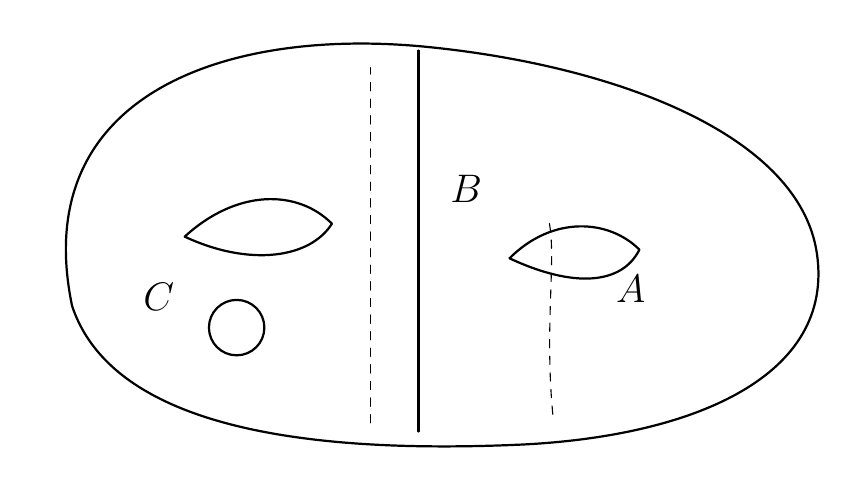
\begin{tikzpicture}[scale=1.1, line cap=round, line join=round]
		
		% Outer boundary of X
		\draw[thick]
		(-4,0) .. controls (-4.5,2.4) and (-2.3,3.2) .. (0,3)
		.. controls (2.2,2.8) and (4.4,2.0) .. (4.6,0.6)
		.. controls (4.8,-0.8) and (3.2,-1.5) .. (1.2,-1.6)
		.. controls (-1.0,-1.7) and (-3.5,-1.5) .. (-4,0);
		
		% Middle separating strip B
		\draw[thick] (0,-1.45) -- (0,2.95);
		\draw[dashed] (-0.55,-1.35) -- (-0.55,2.75);
		
		% Dashed curve in A
		\draw[dashed] (1.55,-1.25) .. controls (1.45,-0.2) and (1.6,0.6) .. (1.5,1.0);
		
		% Schematic loops/holes in C
		\draw[thick]
		(-2.7,0.8) .. controls (-2.1,1.35) and (-1.4,1.35) .. (-1.0,0.95)
		.. controls (-1.25,0.55) and (-1.95,0.45) .. (-2.7,0.8);
		\draw[thick] (-2.1,-0.25) circle (0.32);
		
		% Schematic loop in A
		\draw[thick]
		(1.05,0.55) .. controls (1.55,1.05) and (2.2,1.0) .. (2.55,0.65)
		.. controls (2.35,0.25) and (1.8,0.2) .. (1.05,0.55);
		
		% Labels
		\node at (2.45,0.2) {\Large $A$};
		\node at (0.55,1.35) {\Large $B$};
		\node at (-3.0,0.1) {\Large $C$};
		
	\end{tikzpicture}
	\caption{A schematic decomposition of the genus \(2\) surface \(X=A\cup B\cup C\), where \(A\) and \(C\) are once-punctured tori and \(B\) is the annular strip between them.}
\end{figure}

\begin{figure}[h]
	\centering
	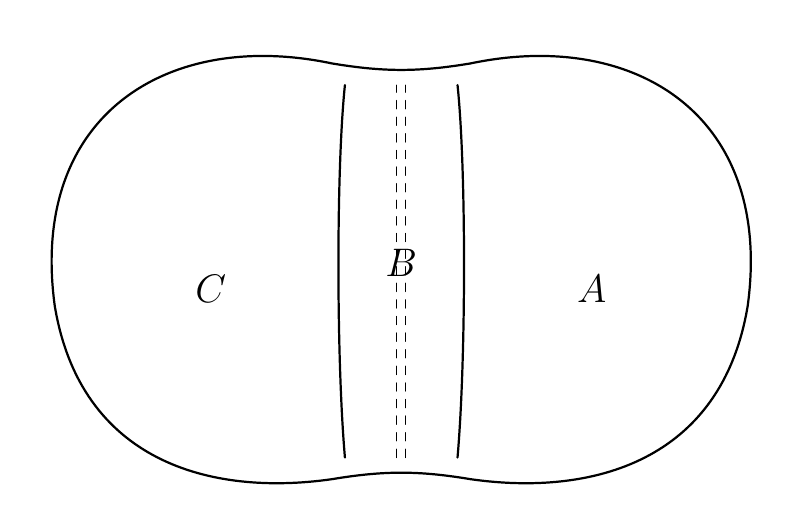
\begin{tikzpicture}[scale=1.1, line cap=round, line join=round]
		
		% Outer boundary of the genus-2 surface (schematic)
		\draw[thick]
		(-4,0) .. controls (-4.3,2.2) and (-2.7,3.2) .. (-0.8,2.8)
		.. controls (-0.2,2.7) and (0.2,2.7) .. (0.8,2.8)
		.. controls (2.7,3.2) and (4.3,2.2) .. (4,0)
		.. controls (3.7,-1.8) and (2.2,-2.2) .. (0.8,-2.0)
		.. controls (0.2,-1.9) and (-0.2,-1.9) .. (-0.8,-2.0)
		.. controls (-2.2,-2.2) and (-3.7,-1.8) .. (-4,0);
		
		% Two cutting circles enclosing the annulus B
		\draw[thick] (-0.65,-1.75) .. controls (-0.75,-0.6) and (-0.75,1.6) .. (-0.65,2.55);
		\draw[thick] ( 0.65,-1.75) .. controls ( 0.75,-0.6) and ( 0.75,1.6) .. ( 0.65,2.55);
		
		% Lightly indicate the annulus strip B
		\draw[dashed] (-0.05,-1.75) -- (-0.05,2.55);
		\draw[dashed] ( 0.05,-1.75) -- ( 0.05,2.55);
		
		% Labels
		\node at (-2.2,0.2) {\Large $C$};
		\node at (0,0.5) {\Large $B$};
		\node at (2.2,0.2) {\Large $A$};
		
	\end{tikzpicture}
\caption{A schematic decomposition of the genus-$2$ surface $X$ into
	$\ensuremath{X = A \cup B \cup C}$, where $\ensuremath{B \cong S^1 \times I}$
	is an annulus and $A$ and $C$ are once-punctured tori.}
	
	
\end{figure}


\begin{figure}[h]
	\centering
	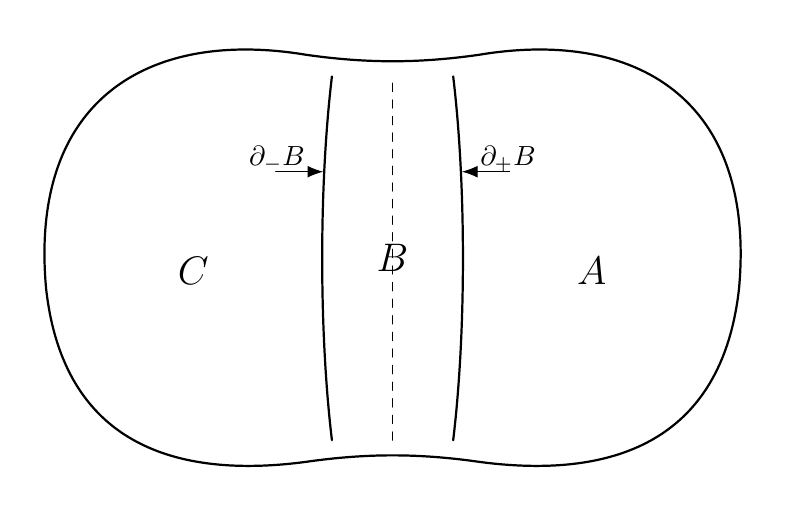
\begin{tikzpicture}[scale=1.1, line cap=round, line join=round]
		
		% Outer boundary of X
		\draw[thick]
		(-4,0) .. controls (-4.2,2.2) and (-2.8,3.0) .. (-1.0,2.7)
		.. controls (-0.3,2.6) and (0.3,2.6) .. (1.0,2.7)
		.. controls (2.8,3.0) and (4.2,2.2) .. (4,0)
		.. controls (3.8,-1.8) and (2.5,-2.2) .. (1.0,-2.0)
		.. controls (0.3,-1.9) and (-0.3,-1.9) .. (-1.0,-2.0)
		.. controls (-2.5,-2.2) and (-3.8,-1.8) .. (-4,0);
		
		% Boundary curves of the annulus B
		\draw[thick] (-0.7,-1.75) .. controls (-0.85,-0.5) and (-0.85,1.2) .. (-0.7,2.45);
		\draw[thick] ( 0.7,-1.75) .. controls ( 0.85,-0.5) and ( 0.85,1.2) .. ( 0.7,2.45);
		
		% Dashed center line to indicate B more clearly
		\draw[dashed] (0,-1.75) -- (0,2.45);
		
		% Labels for the regions
		\node at (-2.3,0.2) {\Large $C$};
		\node at (0,0.35) {\Large $B$};
		\node at (2.3,0.2) {\Large $A$};
		
		% Labels for the boundary components of B
		\node[left] at (-0.9,1.5) {$\partial_- B$};
		\node[right] at (0.9,1.5) {$\partial_+ B$};
		
		% Optional arrows pointing to the boundary components
		\draw[-{Latex[length=2mm]}] (-1.35,1.35) -- (-0.8,1.35);
		\draw[-{Latex[length=2mm]}] (1.35,1.35) -- (0.8,1.35);
		
	\end{tikzpicture}
\caption{A schematic decomposition of the genus-$2$ surface $X$ into
	$\ensuremath{X = A \cup B \cup C}$, where $\ensuremath{B \cong S^1 \times I}$
	is an annulus and $A$ and $C$ are once-punctured tori.}

\end{figure}

The region \(B\) is the strip between the two indicated boundary curves
\(\partial_-B\) and \(\partial_+B\). Since it has exactly two boundary
components, each homeomorphic to \(S^1\), and is topologically a cylinder,
we have
\[
B \cong S^1\times I,
\]
so \(B\) is an annulus.

The complementary regions \(A\) and \(C\) each contain one handle of the
genus \(2\) surface, and each has exactly one boundary circle, namely one of
the boundary components of \(B\). Therefore each of \(A\) and \(C\) is
homeomorphic to a torus with an open disk removed, i.e. a once-punctured
torus:
\[
A \cong T^2\setminus \mathring{D}^2,
\qquad
C \cong T^2\setminus \mathring{D}^2.
\]
Hence \(X\) is decomposed as two once-punctured tori joined by an annulus.

\section{Theory and definitions for Exercise 5}

\subsection{Chain complexes}

A \emph{chain complex} \(C=(C_n,d_n)\) is a sequence of abelian groups (or modules)
\[
\cdots \longrightarrow C_{n+1}\xrightarrow{d_{n+1}} C_n\xrightarrow{d_n} C_{n-1}\xrightarrow{d_{n-1}} \cdots
\]
such that
\[
d_n\circ d_{n+1}=0
\qquad\text{for all }n.
\]
The maps \(d_n\) are called the \emph{boundary maps} or \emph{differentials}.

The condition \(d_n d_{n+1}=0\) means that every boundary is automatically a cycle.

\subsection{Cycles, boundaries, and homology}

For a chain complex \(C\), define
\[
Z_n(C)=\ker(d_n)\subseteq C_n
\]
to be the group of \emph{\(n\)-cycles}, and
\[
B_n(C)=\operatorname{im}(d_{n+1})\subseteq C_n
\]
to be the group of \emph{\(n\)-boundaries}. Since \(d_n d_{n+1}=0\), one has
\[
B_n(C)\subseteq Z_n(C).
\]
The \(n\)-th homology group of \(C\) is
\[
H_n(C)=Z_n(C)/B_n(C)=\ker(d_n)/\operatorname{im}(d_{n+1}).
\]

Homology measures cycles which are not already boundaries.

\subsection{Chain maps}

Let \(C=(C_n,d_n)\) and \(C'=(C'_n,d'_n)\) be chain complexes. A \emph{chain map}
\[
f:C\to C'
\]
is a collection of homomorphisms
\[
f_n:C_n\to C'_n
\]
such that for every \(n\),
\[
d'_n\circ f_n=f_{n-1}\circ d_n.
\]
Equivalently, the squares
\[
\begin{tikzcd}
	C_n \arrow[r,"f_n"] \arrow[d,"d_n"'] & C'_n \arrow[d,"d'_n"] \\
	C_{n-1} \arrow[r,"f_{n-1}"'] & C'_{n-1}
\end{tikzcd}
\]
commute.

A chain map sends cycles to cycles and boundaries to boundaries, and therefore induces homomorphisms on homology:
\[
f_*:H_n(C)\to H_n(C').
\]

\subsection{Chain homotopy}

Two chain maps
\[
f,g:C\to C'
\]
are said to be \emph{chain homotopic}, written
\[
f\sim g,
\]
if there exist homomorphisms
\[
s_n:C_n\to C'_{n+1}
\]
such that
\[
f_n-g_n=d'_{n+1}s_n+s_{n-1}d_n
\qquad\text{for all }n.
\]
This is the algebraic analogue of a homotopy between continuous maps.

A fundamental fact is that chain-homotopic maps induce the same map on homology:
\[
f_*=g_*.
\]

\subsection{Suspension of a chain complex}

If \(C=(C_n,d_n)\) is a chain complex, its \emph{suspension} \(\Sigma C\) is the shifted complex defined by
\[
(\Sigma C)_n=C_{n-1}.
\]
Depending on convention, the differential may carry a sign. For the mapping cone formalism, the sign is chosen so that the exact sequences work correctly.

The key homological identity is
\[
H_n(\Sigma C)\cong H_{n-1}(C).
\]

\subsection{Definition of the mapping cone}

Given a chain map
\[
f:(C,d)\to (C',d'),
\]
its \emph{mapping cone} is the chain complex \(M(f)\) defined degreewise by
\[
M(f)_n=C_{n-1}\oplus C'_n,
\]
with differential
\[
(d_f)_n=
\begin{pmatrix}
	d_{n-1} & 0\\
	(-1)^n f_{n-1} & d'_n
\end{pmatrix}.
\]
Thus on an element \((x,y)\in C_{n-1}\oplus C'_n\),
\[
(d_f)_n(x,y)=\bigl(d_{n-1}x,\; (-1)^n f_{n-1}(x)+d'_n y\bigr).
\]

The mapping cone is built so that it measures the failure of \(f\) to be a homology equivalence.

\subsection{Short exact sequence associated to the cone}

There is a natural short exact sequence of chain complexes
\[
0\longrightarrow C' \xrightarrow{i} M(f)\xrightarrow{p} \Sigma C \longrightarrow 0,
\]
where
\[
i(y)=(0,y),
\qquad
p(x,y)=x.
\]
This exact sequence is one of the main structural reasons why the mapping cone is useful. It yields a long exact sequence in homology:
\[
\cdots \to H_n(C') \to H_n(M(f)) \to H_{n-1}(C)\xrightarrow{f_*} H_{n-1}(C') \to H_{n-1}(M(f)) \to \cdots
\]
and the connecting map is essentially the map induced by \(f\).

\subsection{Acyclic complexes and quasi-isomorphisms}

A chain complex \(K\) is called \emph{acyclic} if all of its homology groups vanish:
\[
H_n(K)=0
\qquad\text{for all }n.
\]
A chain map
\[
f:C\to C'
\]
is called a \emph{quasi-isomorphism} if it induces an isomorphism in every degree:
\[
f_*:H_n(C)\xrightarrow{\cong} H_n(C').
\]
The basic theorem behind Exercise 5 is:

\medskip
\noindent
\textbf{Theorem.}
The mapping cone \(M(f)\) is acyclic if and only if \(f\) is a quasi-isomorphism.

\medskip
Thus the cone is an algebraic device for detecting whether \(f\) preserves all homology.

\subsection{Homotopy invariance of the cone}

If \(f\sim g\), then their mapping cones are chain-isomorphic (hence in particular chain-homotopy equivalent). So the cone depends only on the chain-homotopy class of the map.

This is important conceptually: the mapping cone is not merely attached to a specific formula for \(f\), but to the homotopy-theoretic content of \(f\).

\subsection{Geometric intuition}

The algebraic mapping cone is modeled on the topological mapping cone of a continuous map
\[
F:X\to Y.
\]
In topology one forms
\[
C(F)=\bigl(X\times I \sqcup Y\bigr)\big/\bigl((x,1)\sim F(x),\ (x,0)\sim (x',0)\bigr).
\]
That construction attaches the cone on \(X\) to \(Y\) along the map \(F\).

The chain-level mapping cone plays the same role algebraically: it packages the map \(f\) into a new complex whose homology records how far \(f\) is from being an equivalence.

\bigskip

\section{Theory and definitions for Exercise 6}

\subsection{Pairs of spaces and relative homology}

A \emph{pair of spaces} \((X,A)\) consists of a topological space \(X\) together with a subspace \(A\subseteq X\).

The relative singular chain groups are defined by
\[
C_n(X,A)=C_n(X)/C_n(A).
\]
The differential on \(C_n(X)\) descends to the quotient, so \((C_n(X,A),\partial)\) is again a chain complex. Its homology groups are called the \emph{relative homology groups}:
\[
H_n(X,A)=H_n(C_*(X,A)).
\]

Intuitively, relative homology studies chains in \(X\) while declaring everything in \(A\) to be trivial.

\subsection{Interpretation of relative cycles}

An element of \(H_n(X,A)\) is represented by an \(n\)-chain in \(X\) whose boundary lies in \(A\). Two such chains define the same relative class if they differ by a boundary in \(X\) together with something entirely supported in \(A\).

So relative homology is especially useful when one wants to study what remains of \(X\) after collapsing or ignoring a chosen subspace \(A\).

\subsection{Long exact sequence of a pair}

Every pair \((X,A)\) gives rise to a short exact sequence of chain complexes
\[
0\longrightarrow C_*(A)\longrightarrow C_*(X)\longrightarrow C_*(X,A)\longrightarrow 0,
\]
and hence to the \emph{long exact sequence of the pair}:
\[
\cdots \to H_n(A)\to H_n(X)\to H_n(X,A)\to H_{n-1}(A)\to H_{n-1}(X)\to \cdots
\]
This sequence is the main tool for computing relative homology and for recovering \(H_*(X)\) from \(H_*(A)\) and \(H_*(X,A)\).

In Exercise 6, it is exactly this sequence that allows one to compute \(H_*(X)\) from the pair \((X,A)\).

\subsection{Excision}

A key theorem in relative homology is the \emph{excision theorem}. Roughly speaking, if \(U\subseteq A\subseteq X\) is a suitably nice subspace contained in the interior of \(A\), then removing \(U\) from both \(X\) and \(A\) does not change relative homology:
\[
H_n(X,A)\cong H_n(X\setminus U, A\setminus U).
\]
Excision allows us to replace a complicated pair by a smaller and more convenient one.

In Exercise 6, excision is used to replace \((X,A)\) by a pair homeomorphic to
\[
(Y,\partial Y),
\]
where \(Y\) is a once-punctured torus.

\subsection{Surfaces, genus, and boundary}

A \emph{surface} is a two-dimensional topological manifold. A surface may be closed (compact and without boundary) or may have boundary.

The \emph{genus} of a closed orientable surface is the number of handles. Thus:

\begin{itemize}
	\item genus \(0\): sphere \(S^2\),
	\item genus \(1\): torus \(T^2\),
	\item genus \(2\): double torus,
	\item and so on.
\end{itemize}

The closed orientable surface of genus \(g\) is usually denoted \(\Sigma_g\). Its homology groups are
\[
H_0(\Sigma_g)\cong \mathbb Z,\qquad
H_1(\Sigma_g)\cong \mathbb Z^{2g},\qquad
H_2(\Sigma_g)\cong \mathbb Z.
\]
So for genus \(2\),
\[
H_0(\Sigma_2)\cong \mathbb Z,\qquad
H_1(\Sigma_2)\cong \mathbb Z^4,\qquad
H_2(\Sigma_2)\cong \mathbb Z.
\]

\subsection{The torus and the once-punctured torus}

The torus is
\[
T^2=S^1\times S^1.
\]
A \emph{once-punctured torus} is obtained by removing an open disk:
\[
T^2\setminus \mathring{D}^2.
\]
This is a compact orientable surface with one boundary component.

Its homology groups are
\[
H_0(T^2\setminus \mathring{D}^2)\cong \mathbb Z,\qquad
H_1(T^2\setminus \mathring{D}^2)\cong \mathbb Z^2,\qquad
H_n(T^2\setminus \mathring{D}^2)=0\quad(n\ge 2).
\]
The reason \(H_2\) vanishes is that the surface now has boundary, so it no longer carries a nontrivial absolute fundamental class in dimension \(2\).

\subsection{The annulus}

An \emph{annulus} is any space homeomorphic to
\[
S^1\times I,
\qquad I=[0,1].
\]
Geometrically, this is a cylinder or a planar ring. Its homology groups are
\[
H_0(S^1\times I)\cong \mathbb Z,\qquad
H_1(S^1\times I)\cong \mathbb Z,\qquad
H_n(S^1\times I)=0\quad(n\ge 2).
\]
Thus an annulus has one essential one-dimensional loop and no two-dimensional homology.

\subsection{Boundary of a surface with boundary}

If \(S\) is a compact surface with boundary, then \(\partial S\) is a union of circles. In the case of a once-punctured torus,
\[
\partial\bigl(T^2\setminus \mathring{D}^2\bigr)\cong S^1.
\]
This boundary circle is null-homologous inside the surface, because it is literally the boundary of the surface regarded as a relative \(2\)-chain. Therefore the induced map
\[
H_1(\partial S)\to H_1(S)
\]
is zero for a once-punctured torus.

This fact is used directly in the long exact sequence computations in Exercise 6.

\subsection{Relative homology of a manifold with boundary}

If \(M\) is a compact connected orientable \(2\)-manifold with boundary, then the relative homology group
\[
H_2(M,\partial M)
\]
is isomorphic to \(\mathbb Z\). This is the relative fundamental class of the manifold.

For a once-punctured torus \(T^\circ\),
\[
H_2(T^\circ,\partial T^\circ)\cong \mathbb Z,
\qquad
H_1(T^\circ,\partial T^\circ)\cong \mathbb Z^2,
\qquad
H_0(T^\circ,\partial T^\circ)=0.
\]
These are precisely the groups that appear, via excision, in the computation of \(H_*(X,A)\) and \(H_*(X,C)\).

\subsection{How the genus \(2\) surface is decomposed}

In Exercise 6, the genus \(2\) surface \(X\) is decomposed as
\[
X=A\cup B\cup C,
\]
where:

\begin{itemize}
	\item \(A\) is one once-punctured torus,
	\item \(C\) is the other once-punctured torus,
	\item \(B\cong S^1\times I\) is the annulus joining them.
\end{itemize}

Topologically, this means that the genus \(2\) surface can be understood as two one-handled pieces glued together along a cylindrical band.

This decomposition is useful because the pieces have very simple homology, and relative homology lets us pass from the pieces back to the whole surface.

\subsection{Conceptual summary of Exercise 6}

The strategy behind Exercise 6 is:

\begin{enumerate}
	\item Replace \((X,A)\) by a simpler pair using excision.
	\item Compute the relative homology of a once-punctured torus modulo its boundary.
	\item Use the long exact sequence of the pair \((X,A)\) to reconstruct \(H_*(X)\).
	\item Use symmetry for \(C\).
	\item Use excision and disjoint unions for the pair \((X,B)\).
\end{enumerate}

So the exercise is really an application of three major ideas:

\begin{itemize}
	\item relative homology,
	\item excision,
	\item the long exact sequence of a pair.
\end{itemize}

\subsection{Useful standard facts}

For quick reference, the standard homology groups used in Exercise 6 are:

\[
H_*(S^1):
\qquad
H_0\cong \mathbb Z,\quad H_1\cong \mathbb Z,\quad H_n=0 \ (n\ge 2),
\]
\[
H_*(\text{annulus }S^1\times I):
\qquad
H_0\cong \mathbb Z,\quad H_1\cong \mathbb Z,\quad H_n=0 \ (n\ge 2),
\]
\[
H_*(T^2\setminus \mathring{D}^2):
\qquad
H_0\cong \mathbb Z,\quad H_1\cong \mathbb Z^2,\quad H_n=0 \ (n\ge 2),
\]
\[
H_*(\Sigma_2):
\qquad
H_0\cong \mathbb Z,\quad H_1\cong \mathbb Z^4,\quad H_2\cong \mathbb Z,\quad H_n=0 \ (n\ge 3).
\]

\subsection{Bridge between Exercises 5 and 6}

Although Exercises 5 and 6 look different, they are both based on the same general philosophy of homological algebra:

\begin{itemize}
	\item build a chain complex from the situation,
	\item compare complexes using exact sequences,
	\item read topological information from homology groups.
\end{itemize}

In Exercise 5, the comparison is encoded by the mapping cone of a chain map.

In Exercise 6, the comparison is encoded by the short exact sequence
\[
0\to C_*(A)\to C_*(X)\to C_*(X,A)\to 0
\]
and the resulting long exact sequence in homology.

\subsection{How the pieces \(A\), \(B\), and \(C\) are connected}

The correct topological picture is the following. One starts with two tori and removes one open disk from each of them. This produces two \emph{once-punctured tori}:
\[
A \cong T^2 \setminus \mathring{D}^2,
\qquad
C \cong T^2 \setminus \mathring{D}^2.
\]
Because one open disk has been removed from each torus, each of the spaces \(A\) and \(C\) has exactly one boundary component, and that boundary component is a circle:
\[
\partial A \cong S^1,
\qquad
\partial C \cong S^1.
\]

Next, one takes an annulus
\[
B \cong S^1 \times I,
\qquad I=[0,1].
\]
The annulus has exactly two boundary circles:
\[
\partial B
=
\bigl(S^1\times\{0\}\bigr)\sqcup \bigl(S^1\times\{1\}\bigr).
\]

The genus \(2\) surface is obtained by gluing one boundary circle of the annulus to the boundary circle of \(A\), and the other boundary circle of the annulus to the boundary circle of \(C\). In symbols, the gluing is:
\[
S^1\times\{0\}\sim \partial A,
\qquad
S^1\times\{1\}\sim \partial C.
\]

Thus \(A\) and \(C\) do not meet directly. Instead, they are connected through the annulus \(B\). Topologically, the whole surface is
\[
X=A\cup B\cup C,
\]
where \(A\cap B\cong S^1\), \(B\cap C\cong S^1\), and \(A\cap C=\varnothing\).

\subsection{Why \(A\) and \(C\) are once-punctured tori}

Each of the pieces \(A\) and \(C\) contains one handle and has exactly one boundary component. A compact orientable surface with one handle and one boundary circle is precisely a torus with one open disk removed. Therefore
\[
A \cong T^2\setminus \mathring{D}^2,
\qquad
C \cong T^2\setminus \mathring{D}^2.
\]

\subsection{Why \(B\) is an annulus}

The middle connecting piece \(B\) is a band joining the two punctured tori. Since it has exactly two boundary components, both homeomorphic to \(S^1\), and no additional handles, it is homeomorphic to a cylinder:
\[
B \cong S^1\times I.
\]
This is exactly the definition of an annulus.

\subsection{Conceptual summary}

So the genus \(2\) surface can be understood as
\[
(\text{once-punctured torus})
\;\cup\;
(\text{annulus})
\;\cup\;
(\text{once-punctured torus}).
\]
Equivalently, one may say:

\begin{enumerate}
	\item Start with two tori.
	\item Remove one open disk from each torus.
	\item Take an annulus \(S^1\times I\).
	\item Glue one boundary circle of the annulus to the boundary of the first punctured torus.
	\item Glue the other boundary circle of the annulus to the boundary of the second punctured torus.
\end{enumerate}

The resulting space is the closed orientable surface of genus \(2\).

\subsection{Short version}

A compact way to describe the construction is:
\[
X
=
\bigl(T^2\setminus \mathring{D}^2\bigr)
\cup_{S^1}
\bigl(S^1\times I\bigr)
\cup_{S^1}
\bigl(T^2\setminus \mathring{D}^2\bigr).
\]
That is, the genus \(2\) surface is obtained by gluing an annulus between two once-punctured tori.

\section{Problem 7: Decomposition of \(S^{n+m+1}\) and the homology of \(S^n \times S^m\)}

\subsection{Statement}

Show that \(S^{n+m+1}\) can be decomposed as the union of
\[
S^n \times D^{m+1}
\quad\text{and}\quad
D^{n+1} \times S^m
\]
along their common boundary
\[
S^n \times S^m.
\]
Compute
\[
H_*(S^n \times S^m)
\quad\text{and}\quad
H_*(D^{n+1} \times S^m,\; S^n \times S^m).
\]

\subsection{Solution}

\textbf{Solution.}
A very clean way to see the required decomposition is to start with the product
\[
D^{n+1} \times D^{m+1}.
\]
Since \(D^{n+1} \times D^{m+1}\) is homeomorphic to \(D^{n+m+2}\), its boundary is homeomorphic to \(S^{n+m+1}\). On the other hand,
\[
\partial\bigl(D^{n+1} \times D^{m+1}\bigr)
=
\bigl(\partial D^{n+1} \times D^{m+1}\bigr)
\cup
\bigl(D^{n+1} \times \partial D^{m+1}\bigr).
\]
Because \(\partial D^{n+1} = S^n\) and \(\partial D^{m+1} = S^m\), this becomes
\[
\partial\bigl(D^{n+1} \times D^{m+1}\bigr)
=
\bigl(S^n \times D^{m+1}\bigr)
\cup
\bigl(D^{n+1} \times S^m\bigr).
\]
Their intersection is
\[
\bigl(S^n \times D^{m+1}\bigr)\cap\bigl(D^{n+1} \times S^m\bigr)
=
S^n \times S^m.
\]
Hence
\[
S^{n+m+1}
\cong
\bigl(S^n \times D^{m+1}\bigr)\cup_{\,S^n \times S^m}\bigl(D^{n+1} \times S^m\bigr).
\]

\subsection{Computation of \(H_*(S^n \times S^m)\)}

Since the homology groups of spheres are free abelian, the K\"unneth formula has no \(\operatorname{Tor}\)-term, so
\[
H_k(S^n \times S^m)
\cong
\bigoplus_{p+q=k} H_p(S^n)\otimes H_q(S^m).
\]
Now
\[
H_p(S^n)\cong
\begin{cases}
	\mathbb Z, & p=0,n,\\
	0, & \text{otherwise},
\end{cases}
\qquad
H_q(S^m)\cong
\begin{cases}
	\mathbb Z, & q=0,m,\\
	0, & \text{otherwise}.
\end{cases}
\]
Therefore the only nonzero contributions occur for
\[
(p,q)=(0,0),\ (n,0),\ (0,m),\ (n,m).
\]
Thus
\[
H_k(S^n \times S^m)\cong
\begin{cases}
	\mathbb Z, & k=0,\\[1mm]
	\mathbb Z, & k=n \text{ and } n\neq m,\\[1mm]
	\mathbb Z, & k=m \text{ and } n\neq m,\\[1mm]
	\mathbb Z\oplus \mathbb Z, & k=n=m,\\[1mm]
	\mathbb Z, & k=n+m,\\[1mm]
	0, & \text{otherwise}.
\end{cases}
\]
Equivalently, one may simply say that \(H_*(S^n \times S^m)\) is generated by:
\begin{itemize}
	\item the class of a point in degree \(0\),
	\item the copy of \(S^n \times \{\ast\}\) in degree \(n\),
	\item the copy of \(\{\ast\} \times S^m\) in degree \(m\),
	\item the fundamental class of \(S^n \times S^m\) in degree \(n+m\).
\end{itemize}

\subsection{Computation of \(H_*(D^{n+1} \times S^m,\; S^n \times S^m)\)}

Observe that
\[
(D^{n+1} \times S^m,\; S^n \times S^m)
=
(D^{n+1},S^n)\times S^m
\]
as a relative product situation. Again by the relative K\"unneth formula,
\[
H_k(D^{n+1} \times S^m,\; S^n \times S^m)
\cong
\bigoplus_{p+q=k} H_p(D^{n+1},S^n)\otimes H_q(S^m).
\]
Now the relative homology of the pair \((D^{n+1},S^n)\) is
\[
H_p(D^{n+1},S^n)\cong
\begin{cases}
	\mathbb Z, & p=n+1,\\
	0, & \text{otherwise}.
\end{cases}
\]
Hence
\[
H_k(D^{n+1} \times S^m,\; S^n \times S^m)
\cong
H_{k-(n+1)}(S^m).
\]
Therefore
\[
H_k(D^{n+1} \times S^m,\; S^n \times S^m)
\cong
\begin{cases}
	\mathbb Z, & k=n+1,\\[1mm]
	\mathbb Z, & k=n+m+1,\\[1mm]
	0, & \text{otherwise}.
\end{cases}
\]

\subsection{Conclusion}

We have shown that
\[
S^{n+m+1}
\cong
\bigl(S^n \times D^{m+1}\bigr)\cup_{\,S^n \times S^m}\bigl(D^{n+1} \times S^m\bigr),
\]
and the homology groups are
\[
H_k(S^n \times S^m)\cong
\begin{cases}
	\mathbb Z, & k=0,n,m,n+m
	\text{ (with the degree \(n=m\) case giving } \mathbb Z\oplus\mathbb Z\text{)},\\
	0, & \text{otherwise},
\end{cases}
\]
and
\[
H_k(D^{n+1} \times S^m,\; S^n \times S^m)
\cong
\begin{cases}
	\mathbb Z, & k=n+1,\ n+m+1,\\
	0, & \text{otherwise}.
\end{cases}
\]

\section{Problem 8: The pair \((S^3,K)\) and the complement \(S^3 - K\)}

\subsection{Statement}

Let \(V \subset S^3\) be an open subset of \(S^3\) homeomorphic to
\[
S^1 \times \operatorname{int}(D^2),
\]
and let
\[
K=S^1 \times 0 \subset S^1 \times \operatorname{int}(D^2)\cong V.
\]
Compute
\[
H_*(S^3,K)
\quad\text{and}\quad
H_*(S^3-K).
\]

\subsection{Solution}

\textbf{Solution.}
The space \(K\) is homeomorphic to \(S^1\), so
\[
H_i(K)\cong
\begin{cases}
	\mathbb Z, & i=0,1,\\
	0, & \text{otherwise}.
\end{cases}
\]
Also
\[
H_i(S^3)\cong
\begin{cases}
	\mathbb Z, & i=0,3,\\
	0, & \text{otherwise}.
\end{cases}
\]

\subsection{Computation of \(H_*(S^3,K)\)}

Use the long exact sequence of the pair \((S^3,K)\):
\[
\cdots \to H_i(K)\to H_i(S^3)\to H_i(S^3,K)\to H_{i-1}(K)\to H_{i-1}(S^3)\to \cdots
\]

We now read off the groups degree by degree.

For \(i=3\), we have
\[
H_3(K)\to H_3(S^3)\to H_3(S^3,K)\to H_2(K),
\]
that is,
\[
0\to \mathbb Z \to H_3(S^3,K)\to 0.
\]
Hence
\[
H_3(S^3,K)\cong \mathbb Z.
\]

For \(i=2\), we have
\[
H_2(K)\to H_2(S^3)\to H_2(S^3,K)\to H_1(K)\to H_1(S^3),
\]
that is,
\[
0\to 0 \to H_2(S^3,K)\to \mathbb Z \to 0.
\]
Hence
\[
H_2(S^3,K)\cong \mathbb Z.
\]

For \(i=1\), we get
\[
H_1(S^3)\to H_1(S^3,K)\to H_0(K)\to H_0(S^3),
\]
that is,
\[
0\to H_1(S^3,K)\to \mathbb Z \xrightarrow{\cong} \mathbb Z.
\]
The map \(H_0(K)\to H_0(S^3)\) is an isomorphism because both spaces are connected and \(K\subset S^3\) is nonempty. Therefore
\[
H_1(S^3,K)=0.
\]

Finally,
\[
H_0(S^3,K)=0
\]
for every pair with nonempty subspace in a connected space.

Thus
\[
H_i(S^3,K)\cong
\begin{cases}
	\mathbb Z, & i=3,\\[1mm]
	\mathbb Z, & i=2,\\[1mm]
	0, & \text{otherwise}.
\end{cases}
\]

\subsection{Computation of \(H_*(S^3-K)\)}

To compute the homology of the complement, Alexander duality is the most natural tool. For a compact locally contractible subspace \(K\subset S^3\),
\[
\widetilde H_i(S^3-K)\cong \widetilde H^{\,2-i}(K).
\]
Since \(K\cong S^1\), its reduced cohomology is
\[
\widetilde H^j(K)\cong
\begin{cases}
	\mathbb Z, & j=1,\\
	0, & \text{otherwise}.
\end{cases}
\]
Hence
\[
\widetilde H_i(S^3-K)\cong
\begin{cases}
	\mathbb Z, & 2-i=1,\\
	0, & \text{otherwise},
\end{cases}
\]
so the only nonzero reduced homology group is
\[
\widetilde H_1(S^3-K)\cong \mathbb Z.
\]
Also
\[
\widetilde H_0(S^3-K)\cong \widetilde H^2(K)=0,
\]
so \(S^3-K\) is connected. Therefore
\[
H_i(S^3-K)\cong
\begin{cases}
	\mathbb Z, & i=0,\\[1mm]
	\mathbb Z, & i=1,\\[1mm]
	0, & \text{otherwise}.
\end{cases}
\]

\subsection{Conclusion}

The homology groups are
\[
H_i(S^3,K)\cong
\begin{cases}
	\mathbb Z, & i=3,2,\\
	0, & \text{otherwise},
\end{cases}
\]
and
\[
H_i(S^3-K)\cong
\begin{cases}
	\mathbb Z, & i=0,1,\\
	0, & \text{otherwise}.
\end{cases}
\]
So the complement \(S^3-K\) has the homology of a circle.

\section{Problem 9: A nonvanishing vector field on \(S^n\) and the antipodal map}

\subsection{Statement}

A vector field on \(S^n\) is a continuous map
\[
v:S^n\to \mathbb R^{n+1}
\]
such that
\[
\langle x,v(x)\rangle =0
\qquad\text{for all }x\in S^n.
\]
If \(v(x)\neq 0\) for all \(x\in S^n\), show that \(\operatorname{id}_{S^n}\) is homotopic to the antipodal map
\[
a(x)=-x.
\]
Deduce that if \(S^n\) admits a nonvanishing vector field, then \(n\) is odd.

\subsection{Solution}

\textbf{Solution.}
Assume \(v(x)\neq 0\) for every \(x\in S^n\). Define a normalized vector field
\[
u(x)=\frac{v(x)}{\|v(x)\|}.
\]
Then \(u:S^n\to S^n\) is continuous and still tangent to the sphere, so
\[
\langle x,u(x)\rangle =0
\qquad\text{for all }x\in S^n.
\]
Thus for each \(x\in S^n\), the vectors \(x\) and \(u(x)\) are orthogonal unit vectors in \(\mathbb R^{n+1}\).

Now define
\[
H:S^n\times [0,1]\to S^n
\]
by
\[
H(x,t)=\cos(\pi t)\,x+\sin(\pi t)\,u(x).
\]
We must check that \(H(x,t)\) really lies in \(S^n\). Since \(\|x\|=1\), \(\|u(x)\|=1\), and \(\langle x,u(x)\rangle =0\), we have
\[
\|H(x,t)\|^2
=
\cos^2(\pi t)\|x\|^2
+
\sin^2(\pi t)\|u(x)\|^2
+
2\cos(\pi t)\sin(\pi t)\langle x,u(x)\rangle.
\]
Hence
\[
\|H(x,t)\|^2
=
\cos^2(\pi t)+\sin^2(\pi t)=1.
\]
So \(H(x,t)\in S^n\) for all \((x,t)\).

At the endpoints,
\[
H(x,0)=\cos(0)\,x+\sin(0)\,u(x)=x,
\]
and
\[
H(x,1)=\cos(\pi)\,x+\sin(\pi)\,u(x)=-x.
\]
Therefore \(H\) is a homotopy from the identity map \(\operatorname{id}_{S^n}\) to the antipodal map \(a(x)=-x\).

\subsection{Deduction using the degree}

Homotopic maps \(S^n\to S^n\) have the same degree. Since \(\operatorname{id}_{S^n}\) is homotopic to the antipodal map \(a\), we obtain
\[
\deg(\operatorname{id}_{S^n})=\deg(a).
\]
But
\[
\deg(\operatorname{id}_{S^n})=1,
\]
while the antipodal map has degree
\[
\deg(a)=(-1)^{n+1}.
\]
Thus
\[
1=(-1)^{n+1}.
\]
This happens exactly when \(n+1\) is even, that is, when \(n\) is odd.

Therefore, if \(S^n\) admits a nonvanishing continuous tangent vector field, then \(n\) must be odd.

\subsection{Conclusion}

A nowhere-zero tangent vector field on \(S^n\) gives a homotopy
\[
\operatorname{id}_{S^n}\simeq -\operatorname{id}_{S^n}.
\]
Comparing degrees then forces
\[
(-1)^{n+1}=1,
\]
so \(n\) must be odd.

\section{Theory block for Problems 7--9}

\subsection{What does \(H_*(X)\) mean?}

\textbf{Meaning of the symbol \(H_*(X)\).}
The notation
\[
H_*(X)
\]
does not denote a single group. It is shorthand for the entire graded family of homology groups
\[
H_0(X),\ H_1(X),\ H_2(X),\ \dots .
\]
So when one writes ``compute \(H_*(X)\),'', one means:

\begin{quote}
	Compute all homology groups \(H_k(X)\) for every degree \(k\ge 0\).
\end{quote}

Likewise,
\[
H_*(X,A)
\]
means the whole family of relative homology groups
\[
H_0(X,A),\ H_1(X,A),\ H_2(X,A),\ \dots .
\]

Very often, in practice, almost all of these groups are zero, and only a few degrees are nonzero.

\subsection{What is \(H_k(X)\)?}

\textbf{Idea.}
The group \(H_k(X)\) measures \(k\)-dimensional holes in a space \(X\).

Informally:
\begin{itemize}
	\item \(H_0(X)\) measures connected components.
	\item \(H_1(X)\) measures loops that cannot be shrunk to a point.
	\item \(H_2(X)\) measures closed surfaces that bound nothing inside the space.
	\item Higher \(H_k(X)\) measure higher-dimensional analogues of holes.
\end{itemize}

\textbf{Chain-level definition.}
In singular homology one forms groups \(C_k(X)\) generated by continuous maps
\[
\sigma:\Delta^k\to X
\]
from the standard \(k\)-simplex into \(X\). These are called singular \(k\)-simplices. One defines boundary maps
\[
\partial_k:C_k(X)\to C_{k-1}(X)
\]
satisfying
\[
\partial_{k-1}\circ \partial_k = 0.
\]
Then:

\begin{itemize}
	\item the group of \(k\)-cycles is
	\[
	Z_k(X)=\ker(\partial_k),
	\]
	\item the group of \(k\)-boundaries is
	\[
	B_k(X)=\operatorname{im}(\partial_{k+1}).
	\]
\end{itemize}

Since every boundary has zero boundary, we have
\[
B_k(X)\subseteq Z_k(X).
\]
The \(k\)-th homology group is defined as
\[
H_k(X)=Z_k(X)/B_k(X).
\]

So \(H_k(X)\) records cycles modulo those cycles that already bound something.

\subsection{Relative homology \(H_k(X,A)\)}

\textbf{Idea.}
Relative homology measures what remains in \(X\) after the part \(A\subseteq X\) is treated as negligible or collapsed.

The relative chain group is
\[
C_k(X,A)=C_k(X)/C_k(A),
\]
and its homology is written
\[
H_k(X,A).
\]

A very important example is
\[
H_k(D^{n+1},S^n).
\]
This pair behaves like a single \((n+1)\)-dimensional cell attached along its boundary. Its homology is
\[
H_k(D^{n+1},S^n)\cong
\begin{cases}
	\mathbb Z, & k=n+1,\\
	0, & \text{otherwise}.
\end{cases}
\]

This is one of the key facts used in Problem 7.

\subsection{Reduced homology}

\textbf{Definition.}
Reduced homology \(\widetilde H_k(X)\) is a slight modification of ordinary homology that is especially convenient for connected spaces and for duality theorems.

For a nonempty connected space:
\[
\widetilde H_0(X)=0,
\qquad
\widetilde H_k(X)\cong H_k(X)\ \text{for }k\ge 1.
\]

For example:
\[
H_0(S^1)\cong \mathbb Z,
\qquad
\widetilde H_0(S^1)=0.
\]

Alexander duality is most naturally written using reduced homology and reduced cohomology.

\subsection{Cohomology and why it appears in Alexander duality}

\textbf{Cohomology.}
The cohomology groups \(H^k(X)\) are algebraic invariants dual to homology groups. For spheres and many simple spaces, their groups look numerically the same as homology groups:
\[
H^k(S^n)\cong
\begin{cases}
	\mathbb Z, & k=0,n,\\
	0, & \text{otherwise}.
\end{cases}
\]

For \(S^1\),
\[
H^k(S^1)\cong
\begin{cases}
	\mathbb Z, & k=0,1,\\
	0, & \text{otherwise}.
\end{cases}
\]
Hence the reduced cohomology is
\[
\widetilde H^k(S^1)\cong
\begin{cases}
	\mathbb Z, & k=1,\\
	0, & \text{otherwise}.
\end{cases}
\]

This is exactly what enters Alexander duality in Problem 8.

\subsection{Homology of disks and spheres}

The basic homology groups used repeatedly are:

\[
H_k(D^r)\cong
\begin{cases}
	\mathbb Z, & k=0,\\
	0, & \text{otherwise},
\end{cases}
\]
because a disk is contractible.

For the sphere:
\[
H_k(S^r)\cong
\begin{cases}
	\mathbb Z, & k=0,r,\\
	0, & \text{otherwise}.
\end{cases}
\]

In reduced homology this becomes:
\[
\widetilde H_k(S^r)\cong
\begin{cases}
	\mathbb Z, & k=r,\\
	0, & \text{otherwise}.
\end{cases}
\]

\subsection{The product decomposition of the sphere}

A central geometric fact behind Problem 7 is:
\[
S^{n+m+1}\cong \partial\bigl(D^{n+1}\times D^{m+1}\bigr).
\]
Now the boundary of a product satisfies
\[
\partial(A\times B)= (\partial A\times B)\cup (A\times \partial B).
\]
Applying this with \(A=D^{n+1}\) and \(B=D^{m+1}\), we obtain
\[
\partial\bigl(D^{n+1}\times D^{m+1}\bigr)
=
\bigl(S^n\times D^{m+1}\bigr)\cup \bigl(D^{n+1}\times S^m\bigr),
\]
and their intersection is
\[
S^n\times S^m.
\]

So geometrically, \(S^{n+m+1}\) can be split into two thickened pieces:
\begin{itemize}
	\item one piece looks like \(S^n\) thickened by an \((m+1)\)-disk,
	\item the other looks like \(S^m\) thickened by an \((n+1)\)-disk.
\end{itemize}

Their common boundary is exactly \(S^n\times S^m\).

\subsection{The K\"unneth formula}

\textbf{Purpose.}
The K\"unneth formula computes the homology of a product \(X\times Y\) from the homology of \(X\) and \(Y\).

In the simplest case, when all relevant homology groups are free abelian, it says:
\[
H_k(X\times Y)\cong \bigoplus_{p+q=k} H_p(X)\otimes H_q(Y).
\]

Since spheres have free homology groups, this applies directly to
\[
S^n\times S^m.
\]

Because
\[
H_p(S^n)\neq 0 \iff p=0 \text{ or } p=n,
\]
and
\[
H_q(S^m)\neq 0 \iff q=0 \text{ or } q=m,
\]
the only possible nonzero tensor products come from:
\[
(0,0),\ (n,0),\ (0,m),\ (n,m).
\]
Therefore:
\[
H_k(S^n\times S^m)\cong
\begin{cases}
	\mathbb Z, & k=0,\\
	\mathbb Z, & k=n \text{ if } n\neq m,\\
	\mathbb Z, & k=m \text{ if } n\neq m,\\
	\mathbb Z\oplus \mathbb Z, & k=n=m,\\
	\mathbb Z, & k=n+m,\\
	0, & \text{otherwise}.
\end{cases}
\]

\subsection{Geometric meaning of the generators of \(H_*(S^n\times S^m)\)}

It is very helpful to understand the homology classes geometrically.

\begin{itemize}
	\item Degree \(0\): one copy of \(\mathbb Z\), generated by the class of a point.
	\item Degree \(n\): generated by
	\[
	S^n\times \{\ast\}.
	\]
	\item Degree \(m\): generated by
	\[
	\{\ast\}\times S^m.
	\]
	\item Degree \(n+m\): generated by the fundamental class of the whole product
	\[
	S^n\times S^m.
	\]
\end{itemize}

If \(n=m\), then the degree \(n\) part contains two independent generators:
\[
[S^n\times \{\ast\}]
\quad\text{and}\quad
[\{\ast\}\times S^n].
\]

\subsection{Relative K\"unneth formula in Problem 7}

For the pair
\[
(D^{n+1}\times S^m,\; S^n\times S^m),
\]
one uses the relative version of the K\"unneth formula:
\[
H_k(D^{n+1}\times S^m,\; S^n\times S^m)
\cong
\bigoplus_{p+q=k} H_p(D^{n+1},S^n)\otimes H_q(S^m).
\]
Since
\[
H_p(D^{n+1},S^n)\cong
\begin{cases}
	\mathbb Z, & p=n+1,\\
	0, & \text{otherwise},
\end{cases}
\]
this simply shifts the homology of \(S^m\) upward by \(n+1\):
\[
H_k(D^{n+1}\times S^m,\; S^n\times S^m)\cong H_{k-(n+1)}(S^m).
\]
Hence:
\[
H_k(D^{n+1}\times S^m,\; S^n\times S^m)\cong
\begin{cases}
	\mathbb Z, & k=n+1,\\
	\mathbb Z, & k=n+m+1,\\
	0, & \text{otherwise}.
\end{cases}
\]

\subsection{Why does \(H_k(D^{n+1},S^n)\) look like one top-dimensional cell?}

The pair \((D^{n+1},S^n)\) is the basic model of a space obtained by attaching one \((n+1)\)-dimensional cell along its boundary.

If one collapses \(S^n\subset D^{n+1}\) to a point, one gets
\[
D^{n+1}/S^n \cong S^{n+1}.
\]
So the pair has the homology of one sphere shifted into the relative setting, and therefore only one nonzero relative group remains:
\[
H_{n+1}(D^{n+1},S^n)\cong \mathbb Z.
\]

This is why relative homology is often interpreted as detecting cells.

\subsection{The long exact sequence of a pair}

For every pair \((X,A)\), there is a long exact sequence
\[
\cdots \to H_k(A)\to H_k(X)\to H_k(X,A)\to H_{k-1}(A)\to H_{k-1}(X)\to \cdots
\]
This is one of the most useful tools in algebraic topology.

In Problem 8 we use it with
\[
(X,A)=(S^3,K),
\qquad K\cong S^1.
\]
Since the homology of \(S^3\) and \(S^1\) is known explicitly, the relative groups \(H_k(S^3,K)\) can be read off directly.

\subsection{Detailed computation of \(H_*(S^3,K)\)}

Since
\[
H_i(S^3)\cong
\begin{cases}
	\mathbb Z, & i=0,3,\\
	0, & \text{otherwise},
\end{cases}
\qquad
H_i(K)\cong H_i(S^1)\cong
\begin{cases}
	\mathbb Z, & i=0,1,\\
	0, & \text{otherwise},
\end{cases}
\]
the long exact sequence yields:

\paragraph{Degree \(3\).}
\[
0=H_3(K)\to H_3(S^3)=\mathbb Z\to H_3(S^3,K)\to H_2(K)=0.
\]
So
\[
H_3(S^3,K)\cong \mathbb Z.
\]

\paragraph{Degree \(2\).}
\[
H_2(K)=0\to H_2(S^3)=0\to H_2(S^3,K)\to H_1(K)=\mathbb Z\to H_1(S^3)=0.
\]
Hence
\[
H_2(S^3,K)\cong \mathbb Z.
\]

\paragraph{Degree \(1\).}
\[
H_1(S^3)=0\to H_1(S^3,K)\to H_0(K)=\mathbb Z\to H_0(S^3)=\mathbb Z.
\]
The map \(H_0(K)\to H_0(S^3)\) is an isomorphism because both are connected. Therefore
\[
H_1(S^3,K)=0.
\]

\paragraph{Degree \(0\).}
For a connected space \(X\) and nonempty subspace \(A\subseteq X\),
\[
H_0(X,A)=0.
\]
Thus
\[
H_0(S^3,K)=0.
\]

So the final result is
\[
H_i(S^3,K)\cong
\begin{cases}
	\mathbb Z, & i=3,\\
	\mathbb Z, & i=2,\\
	0, & \text{otherwise}.
\end{cases}
\]

\subsection{Alexander duality}

\textbf{Statement in the case of \(S^n\).}
If \(K\subset S^n\) is compact and locally contractible, then
\[
\widetilde H_i(S^n-K)\cong \widetilde H^{\,n-i-1}(K).
\]

This is a powerful theorem connecting the topology of a subset \(K\) with the topology of its complement.

In Problem 8 we take \(n=3\), so
\[
\widetilde H_i(S^3-K)\cong \widetilde H^{\,2-i}(K).
\]

If \(K\cong S^1\), then
\[
\widetilde H^j(K)\cong
\begin{cases}
	\mathbb Z, & j=1,\\
	0, & \text{otherwise}.
\end{cases}
\]
Therefore
\[
\widetilde H_i(S^3-K)\cong
\begin{cases}
	\mathbb Z, & i=1,\\
	0, & \text{otherwise}.
\end{cases}
\]
and since the reduced \(H_0\) vanishes, the complement is connected. Thus
\[
H_i(S^3-K)\cong
\begin{cases}
	\mathbb Z, & i=0,1,\\
	0, & \text{otherwise}.
\end{cases}
\]

\subsection{Geometric interpretation of \(S^3-K\)}

In Problem 8 the set \(K\) is the core circle of a solid torus. One may think of \(K\) as an unknot in \(S^3\). Its complement is again a solid torus, and a solid torus deformation retracts onto its central circle:
\[
S^3-K \simeq S^1.
\]
This is exactly consistent with the homology computation:
\[
H_0(S^3-K)\cong \mathbb Z,\qquad H_1(S^3-K)\cong \mathbb Z,
\]
and all higher groups vanish.

\subsection{Vector fields on \(S^n\)}

A vector field on \(S^n\) is a continuous map
\[
v:S^n\to \mathbb R^{n+1}
\]
such that for each \(x\in S^n\),
\[
\langle x,v(x)\rangle =0.
\]
This condition means that \(v(x)\) lies in the tangent space of the sphere at \(x\).

Indeed, the tangent space at \(x\in S^n\subset \mathbb R^{n+1}\) is
\[
T_xS^n=\{w\in \mathbb R^{n+1}:\langle x,w\rangle =0\}.
\]

A vector field is called nonvanishing if
\[
v(x)\neq 0\qquad \text{for all }x\in S^n.
\]

\subsection{Normalization of a nonvanishing vector field}

If \(v(x)\neq 0\) everywhere, one may define
\[
u(x)=\frac{v(x)}{\|v(x)\|}.
\]
Then \(u(x)\in S^n\), and because \(v(x)\) is tangent to the sphere, \(u(x)\) is also tangent:
\[
\langle x,u(x)\rangle =0.
\]

So for every \(x\in S^n\), the vectors \(x\) and \(u(x)\) are orthogonal unit vectors.

This gives a very natural path from \(x\) to \(-x\): one simply rotates in the 2-plane spanned by \(x\) and \(u(x)\).

\subsection{The homotopy to the antipodal map}

Define
\[
H:S^n\times [0,1]\to S^n
\]
by
\[
H(x,t)=\cos(\pi t)\,x+\sin(\pi t)\,u(x).
\]
Because \(x\) and \(u(x)\) are orthogonal unit vectors,
\[
\|H(x,t)\|^2=\cos^2(\pi t)+\sin^2(\pi t)=1.
\]
Thus \(H(x,t)\in S^n\).

At the endpoints:
\[
H(x,0)=x,
\qquad
H(x,1)=-x.
\]
Therefore
\[
\operatorname{id}_{S^n}\simeq a,
\]
where \(a(x)=-x\) is the antipodal map.

\subsection{Degree of a map \(S^n\to S^n\)}

\textbf{Definition.}
For a continuous map
\[
f:S^n\to S^n,
\]
the induced map on top homology
\[
f_*:H_n(S^n)\to H_n(S^n)
\]
is multiplication by an integer. Since
\[
H_n(S^n)\cong \mathbb Z,
\]
there exists a unique integer \(\deg(f)\) such that
\[
f_* = \deg(f)\cdot \operatorname{id}_{\mathbb Z}.
\]
This integer is called the degree of \(f\).

\textbf{Important facts.}
\begin{itemize}
	\item \(\deg(\operatorname{id}_{S^n})=1\).
	\item Homotopic maps have the same degree.
	\item The antipodal map \(a(x)=-x\) has degree
	\[
	\deg(a)=(-1)^{n+1}.
	\]
\end{itemize}

Hence, if \(\operatorname{id}_{S^n}\) is homotopic to the antipodal map, then
\[
1=\deg(\operatorname{id}_{S^n})=\deg(a)=(-1)^{n+1},
\]
so \(n\) must be odd.

\subsection{Why is \(\deg(a)=(-1)^{n+1}\)?}

The antipodal map is the restriction of the linear map
\[
-\operatorname{Id}:\mathbb R^{n+1}\to \mathbb R^{n+1}.
\]
Its determinant is
\[
\det(-\operatorname{Id})=(-1)^{n+1}.
\]
This tells us whether orientation is preserved or reversed:
\begin{itemize}
	\item if \(n+1\) is even, the map preserves orientation,
	\item if \(n+1\) is odd, it reverses orientation.
\end{itemize}
Therefore
\[
\deg(a)=(-1)^{n+1}.
\]

\subsection{Consequences for vector fields on spheres}

From the homotopy argument we conclude:

\begin{quote}
	If \(S^n\) admits a nowhere-zero continuous tangent vector field, then \(n\) must be odd.
\end{quote}

This is only a necessary condition, but in fact it is also true that every odd-dimensional sphere admits a nonvanishing tangent vector field. For example:
\begin{itemize}
	\item \(S^1\) admits the obvious tangent field going around the circle,
	\item \(S^3\) admits many nonvanishing vector fields,
	\item \(S^{2m}\) admits no nowhere-zero tangent vector field.
\end{itemize}

This is closely related to the hairy ball theorem, whose most famous special case says:

\begin{quote}
	There is no nowhere-zero continuous tangent vector field on \(S^2\).
\end{quote}

\subsection{Summary of the main tools used in Problems 7--9}

\textbf{Problem 7.}
\begin{itemize}
	\item boundary of a product,
	\item homology of spheres and disks,
	\item K\"unneth formula,
	\item relative homology of \((D^{n+1},S^n)\).
\end{itemize}

\textbf{Problem 8.}
\begin{itemize}
	\item long exact sequence of a pair,
	\item homology of \(S^1\) and \(S^3\),
	\item Alexander duality,
	\item geometric picture of the complement of a core circle in \(S^3\).
\end{itemize}

\textbf{Problem 9.}
\begin{itemize}
	\item tangent vector fields on spheres,
	\item normalization of a nonvanishing field,
	\item explicit homotopy from the identity to the antipodal map,
	\item degree of a self-map of \(S^n\).
\end{itemize}

\subsection{Compact reference table}

\[
H_k(S^r)\cong
\begin{cases}
	\mathbb Z, & k=0,r,\\
	0, & \text{otherwise},
\end{cases}
\qquad
H_k(D^r)\cong
\begin{cases}
	\mathbb Z, & k=0,\\
	0, & \text{otherwise},
\end{cases}
\]
\[
H_k(D^{r},S^{r-1})\cong
\begin{cases}
	\mathbb Z, & k=r,\\
	0, & \text{otherwise},
\end{cases}
\qquad
\widetilde H_k(S^r)\cong
\begin{cases}
	\mathbb Z, & k=r,\\
	0, & \text{otherwise}.
\end{cases}
\]

For Problem 7:
\[
H_k(S^n\times S^m)\cong
\begin{cases}
	\mathbb Z, & k=0,n,m,n+m \text{ in distinct degrees},\\
	\mathbb Z\oplus \mathbb Z, & k=n=m,\\
	0, & \text{otherwise},
\end{cases}
\]
and
\[
H_k(D^{n+1}\times S^m,\; S^n\times S^m)\cong
\begin{cases}
	\mathbb Z, & k=n+1,\ n+m+1,\\
	0, & \text{otherwise}.
\end{cases}
\]

For Problem 8:
\[
H_k(S^3,K)\cong
\begin{cases}
	\mathbb Z, & k=3,2,\\
	0, & \text{otherwise},
\end{cases}
\qquad
H_k(S^3-K)\cong
\begin{cases}
	\mathbb Z, & k=0,1,\\
	0, & \text{otherwise}.
\end{cases}
\]

For Problem 9:
\[
\operatorname{id}_{S^n}\simeq -\operatorname{id}_{S^n}
\quad\Longrightarrow\quad
1=(-1)^{n+1}
\quad\Longrightarrow\quad
n \text{ is odd.}
\]

\section{Problem 10. Homeomorphisms of the torus and the group \(GL(2,\mathbb Z)\)}

\textbf{Statement.}
Suppose \(f:T^2\to T^2\) is a homeomorphism. Show that
\[
f_*:H_1(T^2)\to H_1(T^2)
\]
defines an element of \(GL(2,\mathbb Z)\), and that any element of \(GL(2,\mathbb Z)\) can be realized by a homeomorphism of \(T^2\).

\medskip

\textbf{Solution.}
Recall that
\[
T^2=S^1\times S^1=\mathbb R^2/\mathbb Z^2,
\qquad
H_1(T^2)\cong H_1(S^1)\oplus H_1(S^1)\cong \mathbb Z\oplus \mathbb Z.
\]
Hence \(f_*\) is a homomorphism
\[
f_*:\mathbb Z^2\to \mathbb Z^2.
\]

Since \(f\) is a homeomorphism, it has an inverse \(f^{-1}:T^2\to T^2\). By functoriality of homology,
\[
(f^{-1})_*\circ f_*=(f^{-1}\circ f)_*=(\mathrm{id}_{T^2})_*=\mathrm{id},
\]
and similarly
\[
f_*\circ (f^{-1})_*=\mathrm{id}.
\]
Therefore \(f_*\) is an automorphism of \(\mathbb Z^2\). But
\[
\mathrm{Aut}(\mathbb Z^2)=GL(2,\mathbb Z),
\]
so \(f_*\) defines an element of \(GL(2,\mathbb Z)\).

We now prove the converse. Let
\[
A=\begin{pmatrix}a&b\\ c&d\end{pmatrix}\in GL(2,\mathbb Z).
\]
Then \(A\) is an invertible linear map \(\mathbb R^2\to \mathbb R^2\) with integer entries and determinant \(\pm 1\). Since the entries are integers, we have
\[
A(\mathbb Z^2)\subseteq \mathbb Z^2.
\]
Since \(A\) is invertible over \(\mathbb Z\), in fact
\[
A(\mathbb Z^2)=\mathbb Z^2.
\]
Therefore \(A\) descends to a map on the quotient
\[
\bar A:\mathbb R^2/\mathbb Z^2\to \mathbb R^2/\mathbb Z^2,
\qquad
[x]\mapsto [Ax].
\]
This is well defined: if \(x-y\in \mathbb Z^2\), then
\[
A(x-y)\in \mathbb Z^2,
\]
so \(Ax\) and \(Ay\) represent the same point of \(\mathbb R^2/\mathbb Z^2\).

Since \(A^{-1}\in GL(2,\mathbb Z)\) as well, the inverse map descends too, and \(\bar A\) is a homeomorphism of \(T^2\).

Finally, the standard generators of \(H_1(T^2)\cong \mathbb Z^2\) are represented by the two coordinate circles:
\[
[S^1\times \{*\}],\qquad [\{*\}\times S^1].
\]
The induced map \((\bar A)_*\) on \(H_1(T^2)\) is exactly the matrix \(A\). Thus every element of \(GL(2,\mathbb Z)\) is realized by a homeomorphism of \(T^2\).

\medskip

Therefore:
\[
\boxed{\text{Homeomorphisms of }T^2\text{ induce elements of }GL(2,\mathbb Z),\text{ and every such element is realizable.}}
\]



\section{Problem 11. The mapping torus exact sequence and computations}

\textbf{Statement.}
Let \(f:X\to X\) be a homeomorphism, and let \(Y\) be the quotient of \(X\times [0,1]\) obtained by identifying \((x,0)\) and \((f(x),1)\). Show there is a long exact sequence
\[
\cdots \longrightarrow H_{n+1}(Y)\longrightarrow H_n(X)\xrightarrow{\,1-f_*\,} H_n(X)\longrightarrow H_n(Y)\longrightarrow H_{n-1}(X)\xrightarrow{\,1-f_*\,}H_{n-1}(X)\longrightarrow\cdots
\]
Compute \(H_*(Y)\) in the following cases:
\begin{enumerate}
	\item \(X=S^n\) and \(f\) is the antipodal map;
	\item \(X=T^2=\mathbb R^2/\mathbb Z^2\) and \(f\) is multiplication by
	\[
	A=\begin{pmatrix}3&4\\2&3\end{pmatrix}.
	\]
\end{enumerate}

\medskip

\textbf{Solution.}
The space \(Y\) is the \emph{mapping torus} of \(f\), usually denoted \(T_f\). It is obtained from \(X\times [0,1]\) by gluing the two ends using \(f\):
\[
(x,0)\sim (f(x),1).
\]
There is a standard long exact sequence in homology for the mapping torus, often called the \emph{Wang exact sequence}:
\[
\cdots \longrightarrow H_{n+1}(Y)\longrightarrow H_n(X)\xrightarrow{\,1-f_*\,} H_n(X)\longrightarrow H_n(Y)\longrightarrow H_{n-1}(X)\xrightarrow{\,1-f_*\,}H_{n-1}(X)\longrightarrow\cdots
\]
This is exactly the desired sequence.

A useful reformulation is that for each \(n\) there is a short exact sequence
\[
0\longrightarrow \operatorname{coker}(1-f_*:H_n(X)\to H_n(X))
\longrightarrow H_n(Y)
\longrightarrow \ker(1-f_*:H_{n-1}(X)\to H_{n-1}(X))
\longrightarrow 0.
\]
We now compute the homology in the two cases.

\subsection*{Case 1: \(X=S^n\), \(f\) the antipodal map}

Recall that
\[
H_k(S^n)=
\begin{cases}
	\mathbb Z, & k=0,n,\\
	0, & \text{otherwise}.
\end{cases}
\]
Let \(a:S^n\to S^n\) denote the antipodal map \(a(x)=-x\). Its degree is
\[
\deg(a)=(-1)^{n+1}.
\]
Therefore:
\begin{itemize}
	\item on \(H_0(S^n)\cong \mathbb Z\), we have \(a_*=\mathrm{id}\), since \(S^n\) is connected;
	\item on \(H_n(S^n)\cong \mathbb Z\), we have \(a_*\) equal to multiplication by \((-1)^{n+1}\).
\end{itemize}

Thus on top homology,
\[
1-a_*=1-(-1)^{n+1}.
\]

\paragraph{If \(n\) is odd.}
Then \((-1)^{n+1}=1\), so
\[
1-a_*=0
\]
on \(H_n(S^n)\). Hence
\[
\ker(1-a_*)=\mathbb Z,\qquad \operatorname{coker}(1-a_*)=\mathbb Z.
\]
From the short exact sequence above we obtain:
\[
H_{n+1}(Y)\cong \mathbb Z,
\qquad
H_n(Y)\cong \mathbb Z.
\]
Also \(1-a_*=0\) on \(H_0(S^n)\), so
\[
H_1(Y)\cong \mathbb Z,
\qquad
H_0(Y)\cong \mathbb Z.
\]
All other homology groups vanish, provided \(n>1\). Therefore for odd \(n>1\),
\[
H_k(Y)=
\begin{cases}
	\mathbb Z, & k=0,1,n,n+1,\\
	0, & \text{otherwise}.
\end{cases}
\]

For \(n=1\), the antipodal map on \(S^1\) is rotation by \(\pi\), which is homotopic to the identity, and its mapping torus is a torus. Hence
\[
H_0(Y)\cong \mathbb Z,\qquad
H_1(Y)\cong \mathbb Z^2,\qquad
H_2(Y)\cong \mathbb Z.
\]

\paragraph{If \(n\) is even.}
Then \((-1)^{n+1}=-1\), so
\[
1-a_*=1-(-1)=2
\]
on \(H_n(S^n)\cong \mathbb Z\). Hence
\[
\ker(1-a_*)=0,\qquad \operatorname{coker}(1-a_*)\cong \mathbb Z/2.
\]
Therefore
\[
H_{n+1}(Y)=0,\qquad H_n(Y)\cong \mathbb Z/2.
\]
Again, on \(H_0\) we have \(1-a_*=0\), so
\[
H_1(Y)\cong \mathbb Z,\qquad H_0(Y)\cong \mathbb Z.
\]
All other groups vanish. Thus for even \(n\),
\[
H_k(Y)=
\begin{cases}
	\mathbb Z, & k=0,1,\\
	\mathbb Z/2, & k=n,\\
	0, & \text{otherwise}.
\end{cases}
\]

\paragraph{Conclusion for Case 1.}
For the mapping torus of the antipodal map on \(S^n\):
\[
H_k(Y)=
\begin{cases}
	\mathbb Z, & \text{if $k=0,1,n,n+1$ and $n$ odd and $n>1$,}\\
	\mathbb Z/2, & \text{if $k=n$ and $n$ even,}\\
	\mathbb Z, & \text{if $k=0,1$ and $n$ even,}\\
	0, & \text{otherwise.}
\end{cases}
\]
For \(n=1\), one gets the homology of \(T^2\).

\subsection*{Case 2: \(X=T^2\), \(f\) induced by \(A=\begin{pmatrix}3&4\\2&3\end{pmatrix}\)}

We know
\[
H_0(T^2)\cong \mathbb Z,\qquad
H_1(T^2)\cong \mathbb Z^2,\qquad
H_2(T^2)\cong \mathbb Z.
\]
The induced map on \(H_1(T^2)\) is the matrix \(A\):
\[
f_*|_{H_1}=A.
\]
Also
\[
\det(A)=3\cdot 3-4\cdot 2=1,
\]
so \(f\) preserves orientation. Hence on \(H_2(T^2)\cong \mathbb Z\),
\[
f_*=\mathrm{id}.
\]
On \(H_0(T^2)\cong \mathbb Z\), we also have \(f_*=\mathrm{id}\), since \(T^2\) is connected.

Therefore
\[
1-f_*=
\begin{cases}
	0 & \text{on }H_0(T^2),\\[1ex]
	I-A & \text{on }H_1(T^2),\\[1ex]
	0 & \text{on }H_2(T^2).
\end{cases}
\]
Now
\[
I-A=
\begin{pmatrix}
	1&0\\
	0&1
\end{pmatrix}
-
\begin{pmatrix}
	3&4\\
	2&3
\end{pmatrix}
=
\begin{pmatrix}
	-2&-4\\
	-2&-2
\end{pmatrix}.
\]
Its determinant is
\[
(-2)(-2)-(-4)(-2)=4-8=-4\neq 0,
\]
so \(I-A\) is injective as a homomorphism \(\mathbb Z^2\to \mathbb Z^2\). Hence
\[
\ker(I-A)=0.
\]

To compute the cokernel, we reduce to Smith normal form. Ignoring the harmless sign,
\[
\begin{pmatrix}
	2&4\\
	2&2
\end{pmatrix}
\sim
\begin{pmatrix}
	2&0\\
	0&2
\end{pmatrix},
\]
so
\[
\operatorname{coker}(I-A)\cong \mathbb Z/2\oplus \mathbb Z/2.
\]

We now compute \(H_k(Y)\).

\paragraph{Computation of \(H_3(Y)\).}
From the Wang sequence,
\[
H_3(Y)\cong \ker(1-f_*:H_2(T^2)\to H_2(T^2)).
\]
But \(1-f_*=0\) on \(H_2(T^2)\cong \mathbb Z\), hence
\[
H_3(Y)\cong \mathbb Z.
\]

\paragraph{Computation of \(H_2(Y)\).}
Using the short exact sequence,
\[
0\to \operatorname{coker}(1-f_*:H_2\to H_2)\to H_2(Y)\to \ker(1-f_*:H_1\to H_1)\to 0.
\]
Since \(1-f_*=0\) on \(H_2\), we have
\[
\operatorname{coker}(1-f_*:H_2\to H_2)\cong \mathbb Z,
\]
and since \(\ker(I-A)=0\), we get
\[
0\to \mathbb Z\to H_2(Y)\to 0\to 0.
\]
Therefore
\[
H_2(Y)\cong \mathbb Z.
\]

\paragraph{Computation of \(H_1(Y)\).}
Again,
\[
0\to \operatorname{coker}(I-A)\to H_1(Y)\to \ker(1-f_*:H_0\to H_0)\to 0.
\]
Since \(1-f_*=0\) on \(H_0\cong \mathbb Z\), we have
\[
\ker(1-f_*:H_0\to H_0)\cong \mathbb Z.
\]
Thus
\[
0\to \mathbb Z/2\oplus \mathbb Z/2\to H_1(Y)\to \mathbb Z\to 0.
\]
Because \(\mathbb Z\) is free, this extension splits, so
\[
H_1(Y)\cong \mathbb Z\oplus \mathbb Z/2\oplus \mathbb Z/2.
\]

\paragraph{Computation of \(H_0(Y)\).}
The mapping torus \(Y\) is connected, hence
\[
H_0(Y)\cong \mathbb Z.
\]

\paragraph{Conclusion for Case 2.}
We obtain
\[
H_k(Y)=
\begin{cases}
	\mathbb Z, & k=0,2,3,\\
	\mathbb Z\oplus \mathbb Z/2\oplus \mathbb Z/2, & k=1,\\
	0, & \text{otherwise}.
\end{cases}
\]



\section{Problem 12. Homology of \(X\times S^1\) and of the torus \(T^n\)}

\textbf{Statement.}
If \(H_*(X)\) is a free abelian group, show that
\[
H_*(X\times S^1)\cong H_*(X)\oplus H_{*-1}(X).
\]
(In fact, this is true even if \(H_*(X)\) is not free.) Compute \(H_*(T^n)\).

\medskip

\textbf{Solution.}
We use the K\"unneth theorem.

The homology of the circle is
\[
H_0(S^1)\cong \mathbb Z,\qquad
H_1(S^1)\cong \mathbb Z,\qquad
H_j(S^1)=0 \quad \text{for }j\ge 2.
\]
Since these groups are free, the \(\operatorname{Tor}\)-terms in the K\"unneth formula vanish. Therefore
\[
H_k(X\times S^1)\cong \bigoplus_{i+j=k} H_i(X)\otimes H_j(S^1).
\]
But only the terms \(j=0\) and \(j=1\) survive, so
\[
H_k(X\times S^1)\cong H_k(X)\otimes H_0(S^1)\;\oplus\; H_{k-1}(X)\otimes H_1(S^1).
\]
Since \(H_0(S^1)\cong H_1(S^1)\cong \mathbb Z\), we conclude
\[
H_k(X\times S^1)\cong H_k(X)\oplus H_{k-1}(X).
\]
Equivalently, as graded groups,
\[
H_*(X\times S^1)\cong H_*(X)\oplus H_{*-1}(X).
\]

\medskip

Now compute \(H_*(T^n)\), where
\[
T^n=(S^1)^n.
\]
We proceed inductively. Since
\[
T^n=T^{n-1}\times S^1,
\]
the above formula gives
\[
H_k(T^n)\cong H_k(T^{n-1})\oplus H_{k-1}(T^{n-1}).
\]
Starting from
\[
T^1=S^1,\qquad H_0(S^1)\cong \mathbb Z,\qquad H_1(S^1)\cong \mathbb Z,
\]
one sees that the ranks satisfy Pascal's recursion
\[
\binom{n}{k}=\binom{n-1}{k}+\binom{n-1}{k-1}.
\]
Thus
\[
H_k(T^n)\cong \mathbb Z^{\binom{n}{k}}
\qquad (0\le k\le n),
\]
and
\[
H_k(T^n)=0\qquad (k>n).
\]

So explicitly,
\[
H_0(T^n)\cong \mathbb Z,
\]
\[
H_1(T^n)\cong \mathbb Z^n,
\]
\[
H_2(T^n)\cong \mathbb Z^{\binom{n}{2}},
\]
\[
\cdots
\]
\[
H_n(T^n)\cong \mathbb Z.
\]

Hence the full answer is
\[
\boxed{H_k(T^n)\cong \mathbb Z^{\binom{n}{k}}.}
\]

A useful conceptual reformulation is that
\[
H_*(T^n)\cong \Lambda^*(\mathbb Z^n),
\]
the exterior algebra on \(n\) generators in degree \(1\).



\section{Problem 13. Degree of the product map \(g(x,y)=(f(x),y)\)}

\textbf{Statement.}
Given
\[
f:(D^n,S^{n-1})\to (D^n,S^{n-1}),
\]
define
\[
g:(D^n\times D^m,\partial(D^n\times D^m))\to (D^n\times D^m,\partial(D^n\times D^m))
\]
by
\[
g(x,y)=(f(x),y).
\]
Show that
\[
\deg g=\deg f.
\]

\medskip

\textbf{Solution.}
Recall first that
\[
H_n(D^n,S^{n-1})\cong \mathbb Z.
\]
If \(u\) is a generator of this group, then by definition
\[
f_*(u)=(\deg f)\,u.
\]

Similarly,
\[
H_{n+m}(D^n\times D^m,\partial(D^n\times D^m))\cong \mathbb Z.
\]
We use the relative K\"unneth theorem. Since
\[
(D^n\times D^m,\partial(D^n\times D^m))
\]
is the product of pairs
\[
(D^n,S^{n-1})\times (D^m,S^{m-1}),
\]
there is a natural isomorphism
\[
H_{n+m}(D^n\times D^m,\partial(D^n\times D^m))
\cong
H_n(D^n,S^{n-1})\otimes H_m(D^m,S^{m-1}).
\]
Let
\[
u\in H_n(D^n,S^{n-1}),\qquad v\in H_m(D^m,S^{m-1})
\]
be generators. Then \(u\times v\) is a generator of
\[
H_{n+m}(D^n\times D^m,\partial(D^n\times D^m)).
\]

Now the map \(g\) is just
\[
g=f\times \mathrm{id}_{D^m}.
\]
Hence on relative homology,
\[
g_*(u\times v)=f_*(u)\times (\mathrm{id}_{D^m})_*(v).
\]
Since \((\mathrm{id}_{D^m})_*(v)=v\), we obtain
\[
g_*(u\times v)=((\deg f)u)\times v=(\deg f)(u\times v).
\]
Thus \(g_*\) acts on the top relative homology group by multiplication by \(\deg f\). By definition, this means
\[
\deg g=\deg f.
\]

Therefore
\[
\boxed{\deg(f\times \mathrm{id}_{D^m})=\deg f.}
\]

\section{Problem 14. Cancellation in a chain complex}

\textbf{Statement.}
Suppose \((C,d)\) is a chain complex such that
\[
C_n=C_n'\oplus A,\qquad C_{n-1}=C_{n-1}'\oplus A,
\]
and suppose that the component of
\[
d_n:C_n'\oplus A\longrightarrow C_{n-1}'\oplus A
\]
mapping \(A\) to \(A\) is the identity map. Show that \((C,d)\) is chain homotopy equivalent to a chain complex \((C',d')\), where
\[
C_i'=C_i \quad \text{for } i\neq n,n-1,
\]
\[
C_n'=C_n',\qquad C_{n-1}'=C_{n-1}',
\]
\[
d_i'=d_i \quad \text{for } i\neq n-1,n,n+1,
\]
and \(d'_{n+1}\) is the composition of \(d_{n+1}\) with the projection onto \(C_n'\).

(Hint: use \(d^2=0\) to determine \(d_n'\).)

\medskip

\textbf{Solution.}
This is the standard \emph{cancellation lemma}. The hypothesis says that inside the complex there is a summand of the form
\[
A \xrightarrow{\;\mathrm{id}\;} A,
\]
and such a piece is contractible. The point is to remove it and adjust the neighboring differential accordingly.

Write
\[
d_n:C_n'\oplus A\longrightarrow C_{n-1}'\oplus A
\]
in block form:
\[
d_n=
\begin{pmatrix}
	u & v\\
	w & 1
\end{pmatrix},
\]
where
\[
u:C_n'\to C_{n-1}',\qquad
v:A\to C_{n-1}',\qquad
w:C_n'\to A,
\]
and \(1:A\to A\) is the identity.

We now determine the new differential \(d_n':C_n'\to C_{n-1}'\). Let
\[
d_{n-1}=(p,q):C_{n-1}'\oplus A\to C_{n-2},
\]
and let
\[
d_{n+1}=\binom{r}{s}:C_{n+1}\to C_n'\oplus A.
\]
Since \(d^2=0\), we have
\[
d_{n-1}d_n=0.
\]
Thus
\[
0=(p,q)
\begin{pmatrix}
	u & v\\
	w & 1
\end{pmatrix}
=
\bigl(pu+qw,\;pv+q\bigr).
\]
Hence
\[
q=-pv,
\]
and therefore
\[
pu-pvw=0,
\]
that is,
\[
p(u-vw)=0.
\]

Similarly, from
\[
d_n d_{n+1}=0
\]
we obtain
\[
0=
\begin{pmatrix}
	u & v\\
	w & 1
\end{pmatrix}
\binom{r}{s}
=
\binom{ur+vs}{wr+s}.
\]
So
\[
s=-wr,
\]
and hence
\[
ur-vwr=(u-vw)r=0.
\]

These identities show that the correct new differential is
\[
d_n'=u-vw.
\]
Also, by the statement of the problem,
\[
d'_{n+1}=r,
\]
that is, \(d_{n+1}\) followed by projection onto the \(C_n'\)-summand. The new complex is therefore
\[
\cdots \to C_{n+1}\xrightarrow{\,r\,}C_n'\xrightarrow{\,u-vw\,}C_{n-1}'\xrightarrow{\,p\,}C_{n-2}\to\cdots
\]
and agrees with \(C\) in every other degree.

We now construct explicit chain maps
\[
f:C\to C',
\qquad
g:C'\to C.
\]

For \(i\neq n,n-1\), let \(f_i=g_i=\mathrm{id}\).

In degree \(n\), define
\[
f_n:C_n'\oplus A\to C_n',
\qquad
f_n(x,a)=x,
\]
and
\[
g_n:C_n'\to C_n'\oplus A,
\qquad
g_n(x)=(x,-wx).
\]

In degree \(n-1\), define
\[
f_{n-1}:C_{n-1}'\oplus A\to C_{n-1}',
\qquad
f_{n-1}(y,b)=y-vb,
\]
and
\[
g_{n-1}:C_{n-1}'\to C_{n-1}'\oplus A,
\qquad
g_{n-1}(y)=(y,0).
\]

A direct computation shows that \(f\) and \(g\) are chain maps. For example, in degree \(n\),
\[
f_{n-1}d_n(x,a)
=
f_{n-1}(ux+va,\,wx+a)
=
ux+va-v(wx+a)
=
(u-vw)x
=
d_n' f_n(x,a),
\]
which is exactly the chain map condition.

Next we check that
\[
f\circ g=\mathrm{id}_{C'}.
\]
In degree \(n\),
\[
f_n(g_n(x))=f_n(x,-wx)=x,
\]
and in degree \(n-1\),
\[
f_{n-1}(g_{n-1}(y))=f_{n-1}(y,0)=y.
\]
So indeed \(fg=\mathrm{id}_{C'}\).

It remains to prove that
\[
g\circ f \simeq \mathrm{id}_C.
\]
Define a homotopy \(h:C\to C[1]\) by
\[
h_i=0 \quad \text{for } i\neq n-1,
\]
and
\[
h_{n-1}:C_{n-1}'\oplus A\to C_n'\oplus A,
\qquad
h_{n-1}(y,b)=(0,b).
\]
We now compute \(dh+hd\).

In degree \(n-1\),
\[
(dh+hd)_{n-1}(y,b)=d_n(0,b)=(vb,b).
\]
On the other hand,
\[
(\mathrm{id}-gf)_{n-1}(y,b)
=
(y,b)-g_{n-1}(y-vb)
=
(y,b)-(y-vb,0)
=
(vb,b).
\]

In degree \(n\),
\[
(dh+hd)_n(x,a)=h_{n-1}(d_n(x,a)).
\]
Since
\[
d_n(x,a)=(ux+va,\;wx+a),
\]
we get
\[
h_{n-1}(d_n(x,a))=(0,wx+a).
\]
Also,
\[
(\mathrm{id}-gf)_n(x,a)
=
(x,a)-g_n(f_n(x,a))
=
(x,a)-g_n(x)
=
(x,a)-(x,-wx)
=
(0,a+wx).
\]
These are equal.

In every other degree, both \(dh+hd\) and \(\mathrm{id}-gf\) vanish. Thus
\[
dh+hd=\mathrm{id}_C-gf.
\]
Therefore
\[
gf\simeq \mathrm{id}_C.
\]

We conclude that \(f\) and \(g\) are chain homotopy inverses, so
\[
\boxed{(C,d)\simeq (C',d').}
\]

\medskip

The essential geometric meaning is that a summand
\[
A\xrightarrow{\mathrm{id}}A
\]
is contractible and may be canceled, at the cost of replacing the remaining differential \(u\) by the corrected differential
\[
u-vw.
\]



\section{Problem 15. Acyclic free chain complexes, quasi-isomorphisms, and the Five Lemma}

\textbf{Statement.}
Suppose \(C\) and \(C'\) are free, finitely generated chain complexes over \(\mathbb Z\).

\begin{enumerate}
	\item[(a)] Use Problem 14 to prove that if \(H_*(C)=0\), then \(C\) is contractible.
	\item[(b)] Suppose \(f:C\to C'\) is a chain map. Using Problem 5, show that \(f\) is a chain homotopy equivalence if and only if
	\[
	f_*:H_*(C)\to H_*(C')
	\]
	is an isomorphism.
	\item[(c)] Use Problems 5 and 14 to give a proof of the Five Lemma.
\end{enumerate}

\medskip

\textbf{Solution.}

\subsection*{(a) If \(H_*(C)=0\), then \(C\) is contractible}

We argue by induction on the total rank
\[
N=\sum_i \operatorname{rank}(C_i).
\]
If \(N=0\), then \(C=0\), so the statement is trivial.

Assume \(N>0\). Let \(n\) be the largest index such that
\[
C_n\neq 0.
\]
Then \(C_{n+1}=0\), so
\[
H_n(C)=\ker(d_n)/\operatorname{im}(d_{n+1})=\ker(d_n).
\]
Since \(H_n(C)=0\), it follows that
\[
\ker(d_n)=0,
\]
hence
\[
d_n:C_n\to C_{n-1}
\]
is injective.

Let
\[
B_{n-1}=\operatorname{im}(d_n)\subseteq C_{n-1}.
\]
Because \(C_n\) is free and \(d_n\) is injective, \(B_{n-1}\cong C_n\) is free. Since \(H_{n-1}(C)=0\), we have
\[
Z_{n-1}=B_{n-1}.
\]
Also,
\[
C_{n-1}/B_{n-1}\cong B_{n-2},
\]
and \(B_{n-2}\) is a subgroup of the free abelian group \(C_{n-2}\), hence is free. Therefore the short exact sequence
\[
0\to B_{n-1}\to C_{n-1}\to B_{n-2}\to 0
\]
splits. So there is a decomposition
\[
C_{n-1}\cong C_{n-1}'\oplus B_{n-1}.
\]

Since \(B_{n-1}\cong C_n\), we may identify both with a free abelian group \(A\). Under these identifications,
\[
C_n\cong A,\qquad C_{n-1}\cong C_{n-1}'\oplus A,
\]
and the differential \(d_n\) has \(A\to A\) component equal to the identity.

Thus Problem 14 applies: we may cancel this pair and obtain a smaller chain complex \(D\) such that
\[
C\simeq D.
\]
Since chain homotopy equivalent complexes have isomorphic homology,
\[
H_*(D)\cong H_*(C)=0.
\]
Also the total rank of \(D\) is strictly smaller than that of \(C\). By the induction hypothesis, \(D\) is contractible. Hence \(C\) is contractible as well.

Therefore
\[
\boxed{H_*(C)=0 \implies C \text{ is contractible}.}
\]

\subsection*{(b) A chain map is a chain homotopy equivalence if and only if it induces homology isomorphisms}

Let
\[
f:C\to C'
\]
be a chain map.

\paragraph{Forward implication.}
Assume first that \(f\) is a chain homotopy equivalence. Then there exists a chain map
\[
g:C'\to C
\]
such that
\[
gf\simeq \mathrm{id}_C,\qquad fg\simeq \mathrm{id}_{C'}.
\]
Chain-homotopic maps induce the same map on homology, so
\[
(gf)_*=\mathrm{id}_{H_*(C)},\qquad (fg)_*=\mathrm{id}_{H_*(C')}.
\]
Hence
\[
g_*f_*=\mathrm{id},\qquad f_*g_*=\mathrm{id},
\]
which shows that
\[
f_*:H_*(C)\to H_*(C')
\]
is an isomorphism.

\paragraph{Reverse implication.}
Now assume that
\[
f_*:H_*(C)\to H_*(C')
\]
is an isomorphism.

By Problem 5, the mapping cone \(\operatorname{Cone}(f)\) fits into a long exact sequence in homology, and from that sequence one obtains the standard criterion:
\[
f_* \text{ is an isomorphism } \Longleftrightarrow H_*(\operatorname{Cone}(f))=0.
\]
Thus
\[
H_*(\operatorname{Cone}(f))=0.
\]

Since \(C\) and \(C'\) are free finitely generated chain complexes, the cone \(\operatorname{Cone}(f)\) is also a free finitely generated chain complex. By part (a), every acyclic free finitely generated chain complex is contractible. Therefore
\[
\operatorname{Cone}(f)\text{ is contractible}.
\]

Again by Problem 5, a chain map has contractible mapping cone if and only if it is a chain homotopy equivalence. Hence \(f\) is a chain homotopy equivalence.

So we have proved
\[
\boxed{
	f \text{ is a chain homotopy equivalence }
	\Longleftrightarrow
	f_*:H_*(C)\to H_*(C') \text{ is an isomorphism}.
}
\]

This is the algebraic analogue of the principle that, for sufficiently good objects, a homology equivalence is already a stronger equivalence.

\subsection*{(c) Proof of the Five Lemma}

We now use Problems 5 and 14 to give a proof of the Five Lemma.

Suppose we have a commutative diagram of abelian groups with exact rows:
\[
\begin{array}{ccccccccc}
	A_1 &\longrightarrow& A_2 &\longrightarrow& A_3 &\longrightarrow& A_4 &\longrightarrow& A_5\\
	\downarrow \alpha_1 && \downarrow \alpha_2 && \downarrow \alpha_3 && \downarrow \alpha_4 && \downarrow \alpha_5\\
	B_1 &\longrightarrow& B_2 &\longrightarrow& B_3 &\longrightarrow& B_4 &\longrightarrow& B_5
\end{array}
\]
Assume that the rows are exact and that
\[
\alpha_1,\alpha_2,\alpha_4,\alpha_5
\]
are isomorphisms. We must prove that \(\alpha_3\) is also an isomorphism.

Treat the two rows as chain complexes concentrated in five consecutive degrees. Since the rows are exact, both chain complexes are acyclic. The vertical maps define a chain map
\[
\alpha:A_\bullet\to B_\bullet.
\]
Because both \(A_\bullet\) and \(B_\bullet\) are acyclic, the induced map on homology
\[
\alpha_*:H_*(A_\bullet)\to H_*(B_\bullet)
\]
is automatically an isomorphism, since both sides are zero. By part (b), it follows that \(\alpha\) is a chain homotopy equivalence. Equivalently, its mapping cone
\[
\operatorname{Cone}(\alpha)
\]
is contractible.

Now consider the structure of \(\operatorname{Cone}(\alpha)\). In the degrees corresponding to the first, second, fourth, and fifth columns, the maps
\[
\alpha_1,\alpha_2,\alpha_4,\alpha_5
\]
are isomorphisms. Hence within the mapping cone there appear four pieces of the form
\[
X\xrightarrow{\cong} X.
\]
By repeated application of the cancellation lemma from Problem 14, these pieces may be removed without changing the chain homotopy type.

After carrying out these cancellations, the cone reduces to a two-term complex concentrated in two consecutive degrees:
\[
0\longrightarrow A_3 \xrightarrow{\alpha_3} B_3 \longrightarrow 0.
\]
Because cancellation preserves chain homotopy type, this reduced complex is still contractible, hence acyclic.

But a two-term complex
\[
0\to A_3\xrightarrow{\alpha_3}B_3\to 0
\]
is acyclic if and only if \(\alpha_3\) is both injective and surjective. Indeed,
\[
H=\ker(\alpha_3)
\]
in the left degree, and
\[
H=\operatorname{coker}(\alpha_3)
\]
in the right degree. So acyclicity means
\[
\ker(\alpha_3)=0,\qquad \operatorname{coker}(\alpha_3)=0.
\]
Therefore \(\alpha_3\) is an isomorphism.

This proves the Five Lemma.

\medskip

So the three parts together give the following picture:

\begin{itemize}
	\item free finitely generated acyclic complexes are contractible;
	\item for such complexes, quasi-isomorphisms are the same as chain homotopy equivalences;
	\item the Five Lemma can be proved by passing to a mapping cone and then canceling the obvious isomorphic pieces.
\end{itemize}

The key philosophy is that exactness, cones, and cancellation turn homological information into a strong structural statement about the chain maps themselves.

\subsection{Theory: chain complexes, contractibility, cancellation, mapping cones, and quasi-isomorphisms}

This subsection collects the main algebraic-topological ideas used in Problems 14 and 15. The central theme is that a chain complex can often be simplified without changing its homotopy type, and that mapping cones provide a powerful way to detect when a chain map is an equivalence.

\subsubsection*{1. Chain complexes}

A \emph{chain complex} \((C,d)\) over \(\mathbb Z\) is a sequence of abelian groups and homomorphisms
\[
\cdots \xrightarrow{d_{n+2}} C_{n+1}\xrightarrow{d_{n+1}} C_n\xrightarrow{d_n} C_{n-1}\xrightarrow{d_{n-1}} \cdots
\]
such that for every \(n\),
\[
d_n\circ d_{n+1}=0.
\]
This condition is usually written in the compact form
\[
d^2=0.
\]

The geometric meaning is the familiar principle that \emph{the boundary of a boundary is zero}. In singular or simplicial homology, for example, the boundary of a triangle is a sum of edges, and the boundary of that sum of edges is zero. A chain complex is the algebraic abstraction of this phenomenon.

\subsubsection*{2. Cycles, boundaries, and homology}

Given a chain complex \((C,d)\), the subgroup
\[
Z_n(C)=\ker(d_n)
\]
is called the group of \emph{\(n\)-cycles}, and the subgroup
\[
B_n(C)=\operatorname{im}(d_{n+1})
\]
is called the group of \emph{\(n\)-boundaries}. Since \(d^2=0\), every boundary is automatically a cycle:
\[
B_n(C)\subseteq Z_n(C).
\]

The \(n\)-th homology group of \(C\) is defined by
\[
H_n(C)=Z_n(C)/B_n(C)=\ker(d_n)/\operatorname{im}(d_{n+1}).
\]
Thus homology measures cycles that do not already come from one dimension higher.

Conceptually, homology detects the failure of exactness. If the complex were exact at \(C_n\), then every cycle would already be a boundary, and \(H_n(C)\) would be zero.

\subsubsection*{3. Acyclic complexes}

A chain complex \(C\) is said to be \emph{acyclic} if all of its homology groups vanish:
\[
H_n(C)=0 \qquad \text{for all }n.
\]
Equivalently,
\[
\ker(d_n)=\operatorname{im}(d_{n+1})
\qquad \text{for all }n.
\]
So in an acyclic complex, every cycle is already a boundary.

It is important to distinguish \emph{acyclic} from \emph{contractible}. Every contractible chain complex is acyclic, but in general the converse need not hold. One of the main points of Problem 15 is that for free, finitely generated chain complexes over \(\mathbb Z\), acyclicity is strong enough to imply contractibility.

\subsubsection*{4. Chain maps}

If \((C,d)\) and \((C',d')\) are chain complexes, a \emph{chain map}
\[
f:C\to C'
\]
is a family of homomorphisms
\[
f_n:C_n\to C_n'
\]
such that
\[
d_n' f_n=f_{n-1} d_n
\]
for every \(n\). In other words, the differentials commute with the map:
\[
\begin{array}{ccc}
	C_n & \xrightarrow{d_n} & C_{n-1}\\
	\downarrow f_n && \downarrow f_{n-1}\\
	C_n' & \xrightarrow{d_n'} & C_{n-1}'
\end{array}
\]
is a commutative square.

Because chain maps send cycles to cycles and boundaries to boundaries, they induce homomorphisms on homology:
\[
f_*:H_n(C)\to H_n(C').
\]
This passage from a chain map to the induced maps on homology is one of the basic functorial constructions in homological algebra.

\subsubsection*{5. Chain homotopy}

Let \(f,g:C\to C'\) be chain maps. A \emph{chain homotopy} from \(f\) to \(g\) is a family of homomorphisms
\[
h_n:C_n\to C'_{n+1}
\]
such that
\[
f_n-g_n=d'_{n+1}h_n+h_{n-1}d_n
\]
for every \(n\). In compact notation,
\[
f-g=d'h+hd.
\]
If such a family exists, we write
\[
f\simeq g.
\]

The key fact is that chain-homotopic maps induce the same map on homology:
\[
f\simeq g \qquad \Longrightarrow \qquad f_*=g_*.
\]
Thus chain homotopy is an algebraic notion of equivalence stronger than merely having the same effect on homology.

\subsubsection*{6. Contractible chain complexes}

A chain complex \(C\) is called \emph{contractible} if the identity map is chain homotopic to the zero map. That is, there exist homomorphisms
\[
h_n:C_n\to C_{n+1}
\]
such that
\[
\mathrm{id}_{C_n}=d_{n+1}h_n+h_{n-1}d_n
\]
for all \(n\). Equivalently,
\[
\mathrm{id}_C=dh+hd.
\]

This is the chain-complex analogue of a topological space being contractible. It means that the complex is homotopically trivial.

Every contractible chain complex is acyclic. Indeed, if
\[
\mathrm{id}_C=dh+hd,
\]
then on homology the right-hand side induces the zero map, so the identity on \(H_*(C)\) is zero. This can happen only if
\[
H_*(C)=0.
\]
Hence
\[
\boxed{\text{contractible} \Longrightarrow \text{acyclic}.}
\]

Problem 15(a) proves the converse under the hypothesis that the complex is free and finitely generated.

\subsubsection*{7. Free finitely generated chain complexes}

A chain complex over \(\mathbb Z\) is called \emph{free finitely generated} if each chain group \(C_n\) is a finitely generated free abelian group. Thus for each \(n\),
\[
C_n\cong \mathbb Z^{r_n}
\]
for some nonnegative integer \(r_n\).

This assumption is extremely useful because subgroups of free abelian groups are again free abelian. As a consequence, short exact sequences often split, allowing one to decompose chain groups into direct sums. That decomposition is precisely what is needed in the cancellation argument of Problem 14.

\subsubsection*{8. The cancellation lemma}

Problem 14 is the standard \emph{cancellation lemma}. Suppose that for some \(n\),
\[
C_n=C_n'\oplus A,\qquad C_{n-1}=C_{n-1}'\oplus A,
\]
and that in block form the differential
\[
d_n:C_n'\oplus A\to C_{n-1}'\oplus A
\]
looks like
\[
d_n=
\begin{pmatrix}
	u & v\\
	w & 1
\end{pmatrix},
\]
where the lower-right component
\[
A\to A
\]
is the identity.

This means that the complex contains a piece of the form
\[
A\xrightarrow{\mathrm{id}}A,
\]
and such a piece is contractible. Therefore it should be removable without changing the chain homotopy type.

However, one cannot simply delete it and leave the rest unchanged, because chains may pass through the canceled summand. The correct new differential on the remaining summands is
\[
d_n'=u-vw.
\]
The term \(vw\) records the effect of traveling from \(C_n'\) into \(A\), then across the identity \(A\to A\), and then back into \(C_{n-1}'\). So the new differential is the original one corrected by this detour.

Thus the cancellation lemma says that a contractible identity-piece inside a chain complex may be removed, at the cost of replacing \(u\) by \(u-vw\). This is one of the central simplification tools in homological algebra.

\subsubsection*{9. Why acyclic free complexes are contractible}

Problem 15(a) uses the cancellation lemma inductively. If \(C\) is free, finitely generated, and acyclic, then in the top nonzero degree the differential
\[
d_n:C_n\to C_{n-1}
\]
must be injective, since
\[
H_n(C)=\ker(d_n)=0
\]
when \(C_{n+1}=0\).

Its image is a free subgroup of \(C_{n-1}\), hence splits off as a direct summand. Therefore one can rewrite the complex so that in degrees \(n\) and \(n-1\) there is a direct summand
\[
A\xrightarrow{\mathrm{id}}A.
\]
By cancellation, this piece may be removed. Repeating the argument eventually collapses the entire complex.

So for free finitely generated complexes,
\[
\boxed{\text{acyclic} \Longrightarrow \text{contractible}.}
\]
Together with the earlier implication, this yields
\[
\boxed{\text{acyclic} \Longleftrightarrow \text{contractible}}
\]
in this setting.

\subsubsection*{10. Mapping cone}

Let
\[
f:C\to C'
\]
be a chain map. Its \emph{mapping cone}, denoted \(\operatorname{Cone}(f)\), is a new chain complex constructed so as to measure the defect of \(f\) from being an equivalence.

A standard convention is
\[
\operatorname{Cone}(f)_n=C_n'\oplus C_{n-1},
\]
with differential
\[
d_{\operatorname{Cone}}(y,x)=\bigl(d'y+f(x),-dx\bigr).
\]
One checks directly that
\[
d_{\operatorname{Cone}}^2=0.
\]

The mapping cone fits into a long exact sequence in homology, and from this sequence one obtains the important criterion:
\[
f_*:H_*(C)\to H_*(C') \text{ is an isomorphism }
\Longleftrightarrow
H_*(\operatorname{Cone}(f))=0.
\]
Thus the cone is acyclic exactly when \(f\) is a homology equivalence.

This is the key algebraic mechanism behind Problem 15(b).

\subsubsection*{11. Quasi-isomorphisms}

A chain map
\[
f:C\to C'
\]
is called a \emph{quasi-isomorphism} if it induces isomorphisms on all homology groups:
\[
f_*:H_n(C)\to H_n(C')
\]
is an isomorphism for every \(n\).

In general, a quasi-isomorphism need not be a chain homotopy equivalence. But in the free finitely generated setting of Problem 15, the mapping cone of a quasi-isomorphism is acyclic, hence contractible, and from this one deduces that \(f\) is actually a chain homotopy equivalence. Therefore, in this setting,
\[
\boxed{\text{quasi-isomorphism} \Longleftrightarrow \text{chain homotopy equivalence}.}
\]

This is one of the most important structural consequences of the theory developed in these problems.

\subsubsection*{12. Chain homotopy equivalence}

A chain map
\[
f:C\to C'
\]
is called a \emph{chain homotopy equivalence} if there exists a chain map
\[
g:C'\to C
\]
such that
\[
gf\simeq \mathrm{id}_C,
\qquad
fg\simeq \mathrm{id}_{C'}.
\]
In that case \(C\) and \(C'\) are said to be \emph{chain homotopy equivalent}.

Because chain-homotopic maps induce the same map on homology, every chain homotopy equivalence induces homology isomorphisms. The deep point of Problem 15(b) is that, for free finitely generated complexes, the converse is also true.

\subsubsection*{13. Exact rows and the Five Lemma}

The \emph{Five Lemma} is a classical result about a commutative diagram with exact rows:
\[
\begin{array}{ccccccccc}
	A_1 &\to& A_2 &\to& A_3 &\to& A_4 &\to& A_5\\
	\downarrow && \downarrow && \downarrow && \downarrow && \downarrow \\
	B_1 &\to& B_2 &\to& B_3 &\to& B_4 &\to& B_5
\end{array}
\]
If four of the five vertical maps are isomorphisms, then under the usual hypotheses the fifth is also an isomorphism.

Problems 5, 14, and 15 together provide an elegant homological proof. One regards the two exact rows as acyclic chain complexes and the vertical maps as a chain map between them. Its mapping cone is then acyclic. Since four of the vertical maps are isomorphisms, the cone contains four obvious summands of the form
\[
X\xrightarrow{\cong}X.
\]
By repeated application of the cancellation lemma, these summands can be removed. What remains is essentially the two-term complex
\[
0\to A_3\xrightarrow{\alpha_3}B_3\to 0.
\]
If this reduced complex is acyclic, then \(\alpha_3\) must be both injective and surjective, hence an isomorphism. This proves the Five Lemma.

\subsubsection*{14. Conceptual summary}

Problems 14 and 15 illustrate a very important philosophy in homological algebra:
\[
\text{complicated chain map}
\;\longrightarrow\;
\text{mapping cone}
\;\longrightarrow\;
\text{acyclic complex}
\;\longrightarrow\;
\text{cancellation}
\;\longrightarrow\;
\text{simple algebraic conclusion}.
\]

The central lessons are the following:
\begin{itemize}
	\item homology measures the failure of exactness in a chain complex;
	\item contractible complexes are homotopically trivial;
	\item in the free finitely generated setting, acyclicity already implies contractibility;
	\item mapping cones detect whether a chain map is a homology equivalence;
	\item the cancellation lemma removes identity-type pieces without changing chain homotopy type.
\end{itemize}

Together, these ideas form one of the standard and most effective toolkits for analyzing chain complexes and proving structural results such as Problem 15 and the Five Lemma.

\subsection{Concrete examples for cancellation, mapping cones, and quasi-isomorphisms}

In this subsection we present several explicit examples illustrating the main ideas used in Problems 14 and 15. These examples show concretely how contractible pieces arise inside complexes, how cancellation works in practice, how mapping cones detect failure of equivalence, and why the freeness assumption in Problem 15 is important.

\subsubsection*{1. The smallest contractible chain complex}

Consider the two-term chain complex
\[
0 \longrightarrow \mathbb Z \xrightarrow{\;\mathrm{id}\;} \mathbb Z \longrightarrow 0,
\]
where the left copy of \(\mathbb Z\) is in degree \(1\) and the right copy is in degree \(0\).

Its homology is easy to compute. In degree \(1\),
\[
H_1=\ker(\mathrm{id})=0.
\]
In degree \(0\),
\[
H_0=\mathbb Z/\operatorname{im}(\mathrm{id})=\mathbb Z/\mathbb Z=0.
\]
So the complex is acyclic.

It is also contractible. Define
\[
h_0:\mathbb Z\to \mathbb Z
\]
to be the identity map, and all other \(h_i\) to be zero. Then
\[
dh+hd=\mathrm{id}.
\]
Thus the identity map on the complex is chain homotopic to zero. Therefore this complex is contractible.

This is the fundamental model of a contractible summand:
\[
\boxed{\mathbb Z \xrightarrow{\mathrm{id}} \mathbb Z.}
\]
It is exactly the type of piece that gets removed in the cancellation lemma.

\subsubsection*{2. A larger acyclic complex reduced by cancellation}

Consider the complex
\[
0 \longrightarrow \mathbb Z \xrightarrow{\binom{1}{0}} \mathbb Z^2 \xrightarrow{(0\ \ 1)} \mathbb Z \longrightarrow 0,
\]
with \(\mathbb Z\) in degrees \(2\) and \(0\), and \(\mathbb Z^2\) in degree \(1\).

The differential in degree \(2\) is
\[
d_2(x)=(x,0),
\]
so
\[
\ker(d_2)=0,
\]
hence
\[
H_2=0.
\]

The differential in degree \(1\) is
\[
d_1(a,b)=b.
\]
Its kernel is
\[
\ker(d_1)=\{(a,0):a\in \mathbb Z\}.
\]
But this is precisely the image of \(d_2\), since
\[
\operatorname{im}(d_2)=\{(x,0):x\in \mathbb Z\}.
\]
Therefore
\[
H_1=\ker(d_1)/\operatorname{im}(d_2)=0.
\]

Finally, \(d_1\) is surjective, so
\[
H_0=\mathbb Z/\operatorname{im}(d_1)=0.
\]
Thus the complex is acyclic.

Now write
\[
\mathbb Z^2=\mathbb Z\oplus \mathbb Z.
\]
Then the map
\[
d_1=(0\ \ 1)
\]
has an identity-type component from the second summand \(\mathbb Z\to \mathbb Z\). This means that a contractible piece is present, and one can cancel it. After cancellation, the complex reduces to
\[
0\longrightarrow \mathbb Z \xrightarrow{\mathrm{id}} \mathbb Z \longrightarrow 0,
\]
which is the basic contractible complex from the previous example. That cancels as well, leaving the zero complex.

This example illustrates very concretely how the proof of Problem 15(a) works: an acyclic free complex can be simplified step by step until nothing remains.

\subsubsection*{3. A direct example of the cancellation formula \(u-vw\)}

Consider a two-term complex with
\[
C_1=\mathbb Z\oplus \mathbb Z,\qquad C_0=\mathbb Z\oplus \mathbb Z,
\]
and differential
\[
d_1=
\begin{pmatrix}
	5 & 2\\
	3 & 1
\end{pmatrix}.
\]
We write this in block form as
\[
d_1=
\begin{pmatrix}
	u & v\\
	w & 1
\end{pmatrix},
\]
where
\[
u=5,\qquad v=2,\qquad w=3.
\]
The lower-right entry is the identity on the summand \(A=\mathbb Z\), so the cancellation lemma applies.

The new differential on the reduced complex is
\[
d_1'=u-vw=5-(2)(3)=-1.
\]
Thus after cancellation, the complex becomes
\[
\mathbb Z \xrightarrow{-1} \mathbb Z.
\]

This example is important because it shows explicitly why the reduced differential is not just \(u\). The correction term \(vw\) records the effect of passing through the canceled summand \(A\). So the formula
\[
d_n'=u-vw
\]
has a genuine geometric and algebraic meaning: it subtracts the detour through the identity-piece that has been removed.

\subsubsection*{4. The mapping cone of the identity map}

Let \(C\) be the chain complex concentrated in degree \(0\):
\[
C_0=\mathbb Z,\qquad C_n=0 \text{ for } n\neq 0.
\]
Take
\[
f=\mathrm{id}:C\to C.
\]
The mapping cone \(\operatorname{Cone}(f)\) is then the two-term complex
\[
0\longrightarrow \mathbb Z \xrightarrow{\mathrm{id}} \mathbb Z \longrightarrow 0.
\]
As seen above, this complex is contractible.

This is exactly what one should expect. The identity map is certainly a chain homotopy equivalence, so its mapping cone should be homotopically trivial. Thus the cone of the identity gives the simplest example of the principle
\[
f \text{ equivalence } \Longrightarrow \operatorname{Cone}(f) \text{ contractible}.
\]

\subsubsection*{5. The mapping cone of multiplication by \(2\)}

Now consider the map
\[
f:\mathbb Z\to \mathbb Z,\qquad f(x)=2x,
\]
again viewed as a chain map between complexes concentrated in degree \(0\).

Its mapping cone is
\[
0\longrightarrow \mathbb Z \xrightarrow{2} \mathbb Z \longrightarrow 0.
\]
Let us compute its homology. In degree \(1\),
\[
H_1=\ker(2)=0,
\]
since multiplication by \(2\) on \(\mathbb Z\) is injective. In degree \(0\),
\[
H_0=\mathbb Z/\operatorname{im}(2)=\mathbb Z/2.
\]
Thus
\[
H_*(\operatorname{Cone}(f))\neq 0.
\]

So the cone is not acyclic. Therefore \(f\) is not a quasi-isomorphism. This is a very concrete illustration of the criterion
\[
f_* \text{ is an isomorphism }
\Longleftrightarrow
H_*(\operatorname{Cone}(f))=0.
\]
Here \(f_*\) is multiplication by \(2\) on \(\mathbb Z\), which is not an isomorphism, and the cone detects exactly that failure by producing the nontrivial homology group \(\mathbb Z/2\).

\subsubsection*{6. A quasi-isomorphism from a free resolution}

Consider the two-term complex
\[
0 \longrightarrow \mathbb Z \xrightarrow{2} \mathbb Z \longrightarrow 0,
\]
with the left \(\mathbb Z\) in degree \(1\) and the right \(\mathbb Z\) in degree \(0\). Its homology is
\[
H_1=0,
\qquad
H_0=\mathbb Z/2.
\]
So this complex has the same homology as the complex
\[
0\longrightarrow \mathbb Z/2 \longrightarrow 0
\]
concentrated in degree \(0\).

Define a chain map from the free complex to the latter by taking reduction modulo \(2\) in degree \(0\):
\[
\mathbb Z \to \mathbb Z/2,\qquad x\mapsto \overline{x},
\]
and zero in degree \(1\). This induces an isomorphism on homology, so it is a quasi-isomorphism.

However, the target complex is not free over \(\mathbb Z\). This example shows why the freeness assumption in Problem 15 is important. In general, a quasi-isomorphism need not be a chain homotopy equivalence unless one is in the special free finitely generated setting.

\subsubsection*{7. A direct sum of contractible pieces}

Consider the complex
\[
0 \longrightarrow \mathbb Z^2 \xrightarrow{
	\begin{pmatrix}
		1 & 0\\
		0 & 1
	\end{pmatrix}
} \mathbb Z^2 \longrightarrow 0.
\]
This is simply
\[
0\longrightarrow \mathbb Z^2 \xrightarrow{\mathrm{id}} \mathbb Z^2 \longrightarrow 0,
\]
so it is contractible.

But one can also decompose it as a direct sum of two copies of the basic contractible complex:
\[
\left(0\to \mathbb Z \xrightarrow{\mathrm{id}} \mathbb Z\to 0\right)
\oplus
\left(0\to \mathbb Z \xrightarrow{\mathrm{id}} \mathbb Z\to 0\right).
\]
This example makes clear that contractible complexes can be built from several smaller contractible pieces, and that cancellation may be viewed as removing one such piece at a time.

\subsubsection*{8. A simple chain-complex picture of the Five Lemma}

Consider the exact sequence
\[
0\to \mathbb Z \xrightarrow{\binom{1}{0}} \mathbb Z^2 \xrightarrow{(0\ \ 1)} \mathbb Z \to 0.
\]
Now place two copies of this sequence in a commutative diagram
\[
\begin{array}{ccccccc}
	0 &\to& \mathbb Z &\to& \mathbb Z^2 &\to& \mathbb Z \to 0\\
	&& \downarrow && \downarrow && \downarrow \\
	0 &\to& \mathbb Z &\to& \mathbb Z^2 &\to& \mathbb Z \to 0
\end{array}
\]
where the left and right vertical maps are the identity. If the diagram commutes, then the middle map is forced to be an isomorphism.

From the chain-complex viewpoint, the two rows are acyclic complexes, and the vertical maps form a chain map between them. The mapping cone is therefore acyclic. Because the outer vertical maps are isomorphisms, the cone contains obvious identity-type pieces, which may be canceled using Problem 14. After cancellation, only a small two-term complex involving the middle map remains. Since the reduced complex is still acyclic, the middle map must be an isomorphism.

This gives a concrete algebraic picture behind the proof of the Five Lemma in Problem 15(c).

\subsubsection*{9. The three most useful examples to remember}

Among all the examples above, the following three are the most fundamental.

\paragraph{(i) The basic contractible piece}
\[
0\to \mathbb Z \xrightarrow{\mathrm{id}} \mathbb Z \to 0.
\]
This is the model for cancellation.

\paragraph{(ii) The cone of multiplication by \(2\)}
\[
0\to \mathbb Z \xrightarrow{2} \mathbb Z \to 0,
\]
whose homology is
\[
H_0\cong \mathbb Z/2.
\]
This is the standard example showing how a cone detects the failure of a map to be a homology isomorphism.

\paragraph{(iii) The free resolution of \(\mathbb Z/2\)}
\[
0\to \mathbb Z \xrightarrow{2} \mathbb Z \to 0,
\]
viewed together with the quasi-isomorphism to
\[
0\to \mathbb Z/2 \to 0.
\]
This illustrates why quasi-isomorphisms and chain homotopy equivalences agree only under additional hypotheses such as freeness.

\medskip

Together, these examples give a concrete working picture of the theory behind Problems 14 and 15: cancellation removes contractible identity-pieces, mapping cones detect homological equivalence, and free acyclic complexes can be reduced step by step until nothing remains.

\subsection{Definition and examples of the mapping cone \texorpdfstring{\(\operatorname{Cone}(f)\)}{Cone(f)}}

The mapping cone is one of the most important constructions in homological algebra. It packages a chain map into a new chain complex whose homology measures how far the map is from being an isomorphism on homology.

\subsubsection*{1. Definition of the mapping cone}

Let
\[
f:C_\bullet \to D_\bullet
\]
be a chain map between chain complexes. A standard definition of the \emph{mapping cone} of \(f\), denoted \(\operatorname{Cone}(f)\), is the chain complex given in degree \(n\) by
\[
\operatorname{Cone}(f)_n=D_n\oplus C_{n-1},
\]
with differential
\[
d_{\operatorname{Cone}}(y,x)=\bigl(d_D y+f(x),\,-d_C x\bigr).
\]
Thus an element of \(\operatorname{Cone}(f)_n\) is a pair
\[
(y,x),\qquad y\in D_n,\quad x\in C_{n-1}.
\]

The minus sign in the second component is essential: it ensures that
\[
d_{\operatorname{Cone}}^2=0.
\]

\paragraph{Verification that \(d_{\operatorname{Cone}}^2=0\).}
Let \((y,x)\in \operatorname{Cone}(f)_n\). Then
\[
d_{\operatorname{Cone}}(y,x)=\bigl(d_D y+f(x),\,-d_C x\bigr).
\]
Applying the differential again, we get
\[
d_{\operatorname{Cone}}^2(y,x)
=
d_{\operatorname{Cone}}\bigl(d_D y+f(x),\,-d_C x\bigr).
\]
Hence
\[
d_{\operatorname{Cone}}^2(y,x)
=
\Bigl(d_D(d_D y+f(x))+f(-d_C x),\,-d_C(-d_C x)\Bigr).
\]
Using \(d_D^2=0\), \(d_C^2=0\), and the chain map identity
\[
d_D f=f d_C,
\]
we obtain
\[
d_{\operatorname{Cone}}^2(y,x)
=
\bigl(0+d_D f(x)-f d_C(x),\,0\bigr)
=
(0,0).
\]
So \(\operatorname{Cone}(f)\) is indeed a chain complex.

\subsubsection*{2. Why the mapping cone is important}

The cone measures the defect of \(f\) from being a homological equivalence. The basic principle is:
\[
f_*:H_*(C)\to H_*(D)\text{ is an isomorphism}
\quad\Longleftrightarrow\quad
H_*(\operatorname{Cone}(f))=0.
\]
So the cone is acyclic exactly when \(f\) is a quasi-isomorphism.

If \(f\) is even stronger, namely a chain homotopy equivalence, then \(\operatorname{Cone}(f)\) is contractible. Thus the cone is the natural object that detects whether a chain map behaves like an equivalence.

\subsubsection*{3. Geometric intuition}

The terminology comes from topology. If \(f:X\to Y\) is a continuous map, one forms the topological mapping cone by attaching the cone on \(X\) to \(Y\) along \(f\). Algebraically, the chain complex
\[
\operatorname{Cone}(f)_n=D_n\oplus C_{n-1}
\]
plays the same role: it consists of the target complex \(D\) together with a shifted copy of the source complex \(C\). The shift reflects the extra cone direction.

Thus one may think of the mapping cone as
\[
\text{target} + \text{shifted source}.
\]

\subsubsection*{4. The cone of the identity map}

Let \(C\) be the chain complex concentrated in degree \(0\):
\[
C_0=\mathbb Z,\qquad C_n=0 \text{ for } n\neq 0.
\]
Take the identity map
\[
f=\mathrm{id}:C\to C.
\]

Then
\[
\operatorname{Cone}(f)_1=C_0=\mathbb Z,
\qquad
\operatorname{Cone}(f)_0=C_0=\mathbb Z,
\]
and all other groups are zero. The only nontrivial differential is
\[
d_1:\mathbb Z\to \mathbb Z.
\]
Let \(x\in \mathbb Z=\operatorname{Cone}(f)_1\). Then in the cone description it corresponds to \((0,x)\), so
\[
d_1(x)=f(x)=x.
\]
Thus
\[
\operatorname{Cone}(\mathrm{id})=
0\longrightarrow \mathbb Z \xrightarrow{\mathrm{id}} \mathbb Z \longrightarrow 0.
\]

This is the basic contractible complex. Hence
\[
\operatorname{Cone}(\mathrm{id})
\]
is contractible.

This is exactly what one expects: the identity map is already a perfect equivalence, so its cone should be trivial from the homotopy viewpoint.

\subsubsection*{5. The cone of the zero map}

Now take the same complexes \(C=D\), concentrated in degree \(0\), but let
\[
f=0:C\to D.
\]
Then again
\[
\operatorname{Cone}(0)_1=\mathbb Z,
\qquad
\operatorname{Cone}(0)_0=\mathbb Z,
\]
but now the differential is zero:
\[
d_1=0.
\]
So
\[
\operatorname{Cone}(0)=
0\longrightarrow \mathbb Z \xrightarrow{0} \mathbb Z \longrightarrow 0.
\]

Its homology is
\[
H_1\cong \mathbb Z,
\qquad
H_0\cong \mathbb Z.
\]
Therefore this cone is very far from acyclic.

This matches the fact that the zero map certainly does not induce an isomorphism on homology.

\subsubsection*{6. The cone of multiplication by \(2\)}

Consider the chain map
\[
f:\mathbb Z\to \mathbb Z,\qquad f(x)=2x,
\]
again viewing both copies of \(\mathbb Z\) as complexes concentrated in degree \(0\).

Then the cone is the two-term complex
\[
\operatorname{Cone}(f)=
0\longrightarrow \mathbb Z \xrightarrow{2} \mathbb Z \longrightarrow 0.
\]

Let us compute its homology. In degree \(1\),
\[
H_1=\ker(2)=0,
\]
since multiplication by \(2\) is injective on \(\mathbb Z\). In degree \(0\),
\[
H_0=\mathbb Z/\operatorname{im}(2)=\mathbb Z/2.
\]
Thus
\[
H_*(\operatorname{Cone}(f))\neq 0.
\]

So \(f\) is not a quasi-isomorphism. The cone detects the precise defect: the cokernel \(\mathbb Z/2\) appears as homology.

This is one of the most important examples to remember.

\subsubsection*{7. The cone of an isomorphism}

Suppose
\[
f:C\to D
\]
is a chain isomorphism. Then \(\operatorname{Cone}(f)\) is contractible.

For example, let
\[
f:\mathbb Z^2\to \mathbb Z^2
\]
be an invertible matrix, such as
\[
\begin{pmatrix}
	1&0\\
	0&1
\end{pmatrix}
\qquad\text{or}\qquad
\begin{pmatrix}
	0&1\\
	1&0
\end{pmatrix}.
\]
Viewed as a chain map between complexes concentrated in degree \(0\), its cone is
\[
0\longrightarrow \mathbb Z^2 \xrightarrow{f} \mathbb Z^2 \longrightarrow 0.
\]
Because \(f\) is an isomorphism, the homology vanishes, and in fact the complex is contractible.

Thus cones of genuine isomorphisms behave just like cones of the identity map: they are homotopically trivial.

\subsubsection*{8. A cone of a quasi-isomorphism that is not a chain isomorphism}

Consider the free complex
\[
0 \longrightarrow \mathbb Z \xrightarrow{2} \mathbb Z \longrightarrow 0,
\]
with the left copy in degree \(1\) and the right copy in degree \(0\). Its homology is
\[
H_1=0,
\qquad
H_0=\mathbb Z/2.
\]

Now compare it with the complex
\[
0\longrightarrow \mathbb Z/2 \longrightarrow 0
\]
concentrated in degree \(0\). Define a chain map by reduction modulo \(2\) in degree \(0\):
\[
\mathbb Z\to \mathbb Z/2,\qquad x\mapsto \overline{x},
\]
and zero in degree \(1\).

This map induces an isomorphism on homology, so it is a quasi-isomorphism. Therefore
\[
H_*(\operatorname{Cone}(f))=0.
\]
So the cone is acyclic.

This example is important because the map is not an isomorphism of chain groups, yet its cone is still acyclic. Thus the cone detects homological equivalence, not literal equality of complexes.

\subsubsection*{9. Cone as target plus shifted source}

Another useful example is obtained by taking a map
\[
f:C\to 0
\]
from a complex \(C\) to the zero complex. Then
\[
\operatorname{Cone}(f)_n=0\oplus C_{n-1}\cong C_{n-1}.
\]
So the cone is just a shift of \(C\):
\[
\operatorname{Cone}(f)\cong C[-1].
\]

For instance, if
\[
C=
\left(0\to \mathbb Z \xrightarrow{\mathrm{id}} \mathbb Z \to 0\right),
\]
then
\[
\operatorname{Cone}(C\to 0)\cong C[-1].
\]
Since \(C\) is contractible, the shifted complex is also contractible.

This example helps one remember the shape of the cone:
\[
\operatorname{Cone}(f)=D\oplus C[-1].
\]

\subsubsection*{10. The exact sequence associated to the cone}

There is a short exact sequence of chain complexes
\[
0\longrightarrow D \longrightarrow \operatorname{Cone}(f)\longrightarrow C[-1]\longrightarrow 0,
\]
where \(C[-1]\) denotes the shifted complex defined by
\[
C[-1]_n=C_{n-1}.
\]
From this short exact sequence one obtains the long exact sequence in homology
\[
\cdots \to H_n(D)\to H_n(\operatorname{Cone}(f))\to H_{n-1}(C)\xrightarrow{\,f_*\,} H_{n-1}(D)\to H_{n-1}(\operatorname{Cone}(f))\to\cdots
\]

This exact sequence is the fundamental reason why the mapping cone detects quasi-isomorphisms. If \(f_*\) is an isomorphism, then exactness forces
\[
H_n(\operatorname{Cone}(f))=0
\]
for all \(n\). Conversely, if the cone is acyclic, then the same exact sequence shows that \(f_*\) must be an isomorphism.

\subsubsection*{11. The most important examples to remember}

Among all examples, the following three are the most useful.

\paragraph{(i) Cone of the identity}
\[
\operatorname{Cone}(\mathrm{id})=
0\to \mathbb Z \xrightarrow{\mathrm{id}} \mathbb Z \to 0,
\]
which is contractible.

\paragraph{(ii) Cone of the zero map}
\[
\operatorname{Cone}(0)=
0\to \mathbb Z \xrightarrow{0} \mathbb Z \to 0,
\]
whose homology is
\[
H_1\cong \mathbb Z,\qquad H_0\cong \mathbb Z.
\]

\paragraph{(iii) Cone of multiplication by \(2\)}
\[
\operatorname{Cone}(2)=
0\to \mathbb Z \xrightarrow{2} \mathbb Z \to 0,
\]
whose homology is
\[
H_0\cong \mathbb Z/2.
\]

These three examples already show the whole philosophy:
\begin{itemize}
	\item the identity map gives a contractible cone;
	\item the zero map gives a highly nontrivial cone;
	\item multiplication by \(2\) gives a cone whose homology records the failure of the map to be an isomorphism.
\end{itemize}

\subsubsection*{12. Conceptual summary}

The mapping cone construction converts a chain map
\[
f:C\to D
\]
into a single chain complex
\[
\operatorname{Cone}(f)
\]
whose homology measures the defect of \(f\). In this way, questions about whether \(f\) is a homology equivalence become questions about whether a certain chain complex is acyclic.

This is why the mapping cone is so powerful in Problems 5, 14, and 15:
\[
\text{chain map}
\;\longrightarrow\;
\text{mapping cone}
\;\longrightarrow\;
\text{acyclicity or contractibility}
\;\longrightarrow\;
\text{strong conclusion about }f.
\]

Thus \(\operatorname{Cone}(f)\) is one of the central bridge constructions between algebraic structure and homological information.

\end{document}


